\documentclass[xcolor=table, aspectratio=1610,ignorenonframetext]{beamer}

%\usepackage{arev}
\usepackage{amsmath,amssymb,amscd}
\usepackage{dsfont}
\usepackage{mathrsfs}
\usepackage{yfonts}
\usepackage{bm}
\usepackage{graphicx}
\usepackage{tabularx}
\usepackage{animate}
\usepackage{listings}
%\usepackage{ifthen}
\usepackage{pifont}

\usepackage{xeCJK}
\usepackage{fontspec}
\newfontfamily\cjkfont{WenQuanYi Zen Hei}
\setCJKmainfont{WenQuanYi Zen Hei}
%\newfontfamily\cjkfont{PingFang SC}
%\setCJKmainfont{PingFang SC}
\newcolumntype{x}{>{\centering\arraybackslash}X}
\renewcommand{\arraystretch}{1.5}
\DeclareMathOperator{\img}{img}
\DeclareMathOperator{\hhom}{Hom}
\newcommand{\uone}{\text U(1)}
\DeclareMathOperator{\id}{id}
\usepackage{tikz}
  \usetikzlibrary{calc}
  \usetikzlibrary{arrows,shapes, positioning, matrix}
	\usetikzlibrary{decorations.markings}
	\tikzstyle arrowstyle=[scale=1]
  \tikzstyle string=[thick,postaction={decorate,decoration={markings,
      mark=at position .55 with {\arrow[arrowstyle]{stealth}}}}]

\usepackage{tikz-cd}
\usepackage{pgffor}
\newcommand{\cohosub}[1]{\scalebox{0.72}{\textswab{#1}}}
\newcommand{\cohosubsub}[1]{\scalebox{0.6}{\textswab{#1}}}
\newcommand{\coho}[1]{\textswab{#1}}


\mode<presentation>
{
  %\usetheme{Warsaw}
  % or ...
  %\useoutertheme{rectangle}
  \setbeamertemplate{frametitle}[default][center]
  \defbeamertemplate{itemize item}{flat}{\begin{pgfpicture}{-1ex}{0ex}{1ex}{2ex}
      \pgfpathcircle{\pgfpoint{0pt}{.6ex}}{0.6ex}
      \pgfusepath{fill}
    \end{pgfpicture}%
  }
  \defbeamertemplate{itemize subitem}{flat}{\footnotesize\raise0.5pt\hbox{\textbullet}}
  \defbeamertemplate{itemize subsubitem}{flat}{\footnotesize\raise0.5pt\hbox{\textbullet}}

  %\useinnertheme{circles}
  \setbeamertemplate{items}[flat]
  \setbeamertemplate{sections/subsections in toc}[circle]
  \setbeamertemplate{blocks}[rounded]
  \setbeamertemplate{title page}[default][colsep=-4bp,rounded=true]
  \setbeamertemplate{part page}[default][colsep=-4bp,rounded=true]
  \setbeamercovered{transparent}
  %\usecolortheme{spruce}
  %\definecolor{THU}{RGB}{116,61,130}
  \definecolor{mbg}{RGB}{0,0,160}
  \setbeamercolor*{palette primary}{fg=white,bg=mbg}
  \setbeamercolor*{titlelike}{parent=palette primary}
  \setbeamercolor*{structure}{fg=mbg}
  \setbeamercolor{frametitle}{fg=white,bg=mbg}
  % or whatever (possibly just delete it)
  \setbeamercolor{block title}{bg=mbg,fg=white}
  \setbeamercolor{block body}{bg=mbg!15}


  \addtobeamertemplate{navigation symbols}{}{ \hspace{1em}%
    \usebeamerfont{footline}%
    \insertframenumber / \inserttotalframenumber }
}


%\usepackage[english]{babel}
% or whatever

%\usepackage[latin1]{inputenc}
% or whatever

%\usepackage{times}
%\usepackage[T1]{fontenc}
% Or whatever. Note that the encoding and the font should match. If T1
% does not look nice, try deleting the line with the fontenc.

\title % (optional, use only with long paper titles)
{Emergent U(1) symmetry and BKT transition in a triangular-lattice quantum Ising material TmMgGaO${}_4$}
\author[Y Qi] % (optional, use only with lots of authors)
{Yang~Qi}
% - Give the names in the same order as the appear in the paper.
% - Use the \inst{?} command only if the authors have different
%   affiliation.

\institute[Fudan] % (optional, but mostly needed)
{
Department of Physics, Fudan University.
}
% - Use the \inst command only if there are several affiliations.
% - Keep it simple, no one is interested in your street address.

%\date{2016 Annual Meeting of Fudan CFTPP} % (optional, should be abbreviation of conference name)
%{Fudan University, Oct 13 2015}
\date{Kavli Institute for Theoretical Sciences, University of Chinese Acamedy of Sciences\\ Nov. 9th, 2020.}
% - Either use conference name or its abbreviation.
% - Not really informative to the audience, more for people (including
%   yourself) who are reading the slides online

%\subject{Theoretical Physics}
% This is only inserted into the PDF information catalog. Can be left
% out.



% If you have a file called "university-logo-filename.xxx", where xxx
% is a graphic format that can be processed by latex or pdflatex,
% resp., then you can add a logo as follows:

\pgfdeclareimage[height=1cm]{university-logo}{../resources/fudan}
\logo{\pgfuseimage{university-logo}}



% Delete this, if you do not want the table of contents to pop up at
% the beginning of each subsection:
\AtBeginSection[]
{
  \begin{frame}<beamer>{Outline}
			\tableofcontents[currentsection,currentsubsection]
  \end{frame}
}
%\AtBeginSubsection[]
%{
 % \begin{frame}<beamer>{Outline}
  %  \tableofcontents[currentsection,currentsubsection]
  %\end{frame}
%}


\begin{document}

\begin{frame}
  \titlepage
\end{frame}

\begin{frame}{Collaborators: Beihang University}
\begin{itemize}
	\item XTRG: Han Li (李涵), Bin-Bin Chen (陈斌斌), Wei Li (李伟).
	\item DFT: Xu-Tao Zeng (曾旭涛), Xian-Lei Sheng (胜献雷).
\end{itemize}
	\begin{center}
		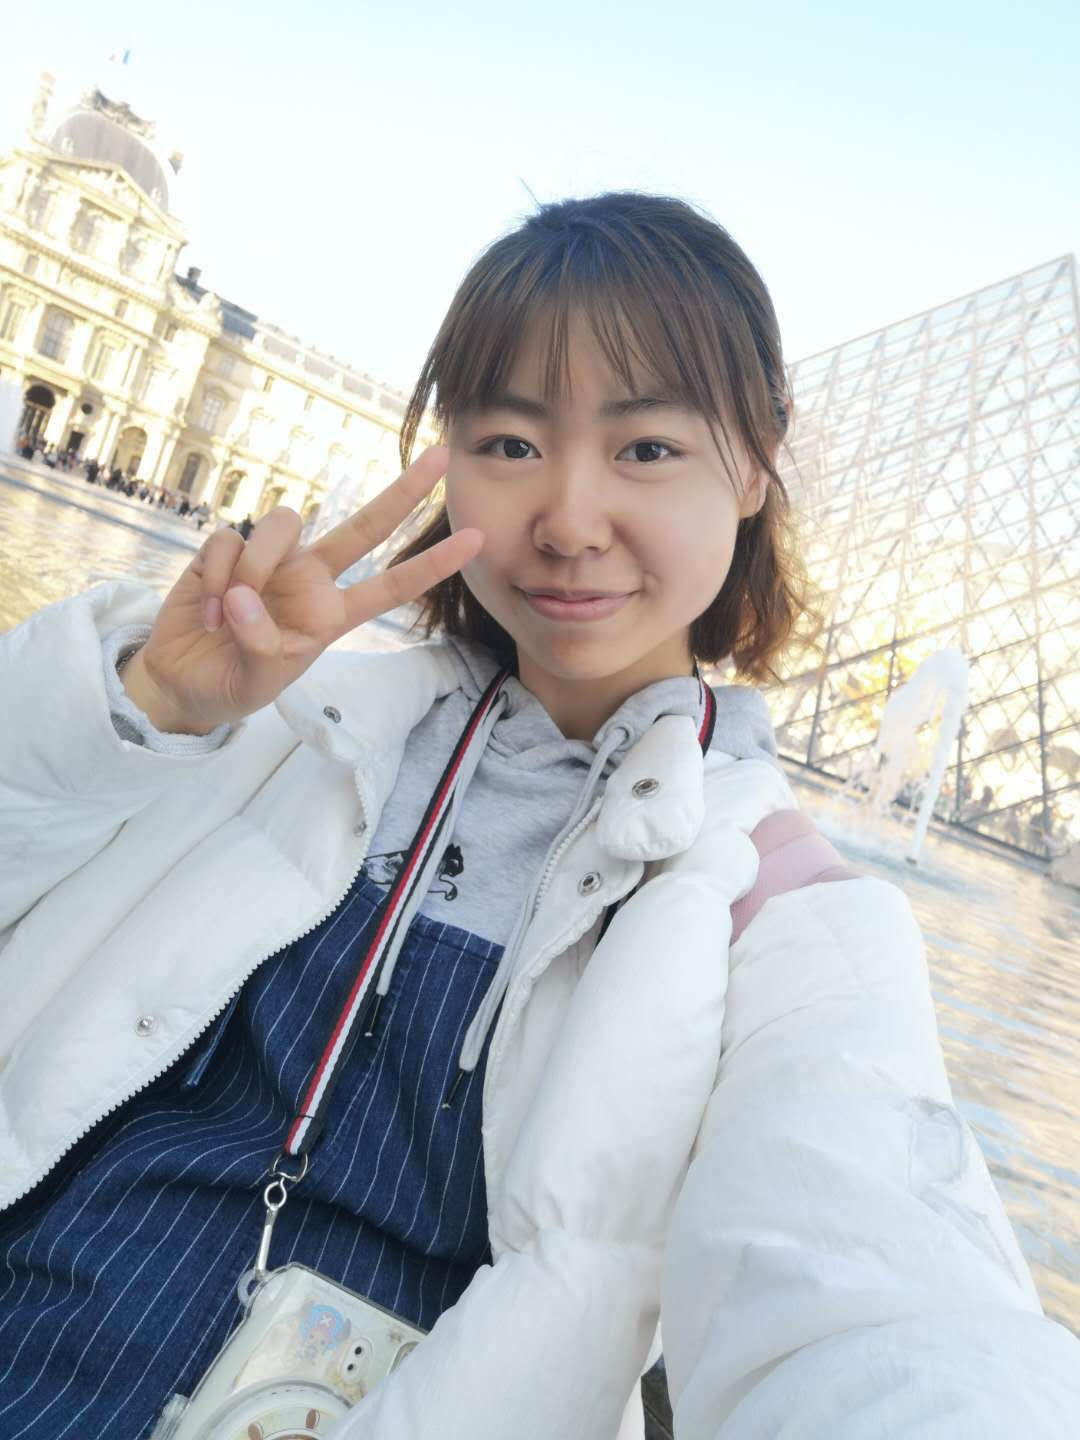
\includegraphics[height=3cm]{../people/hanli}
		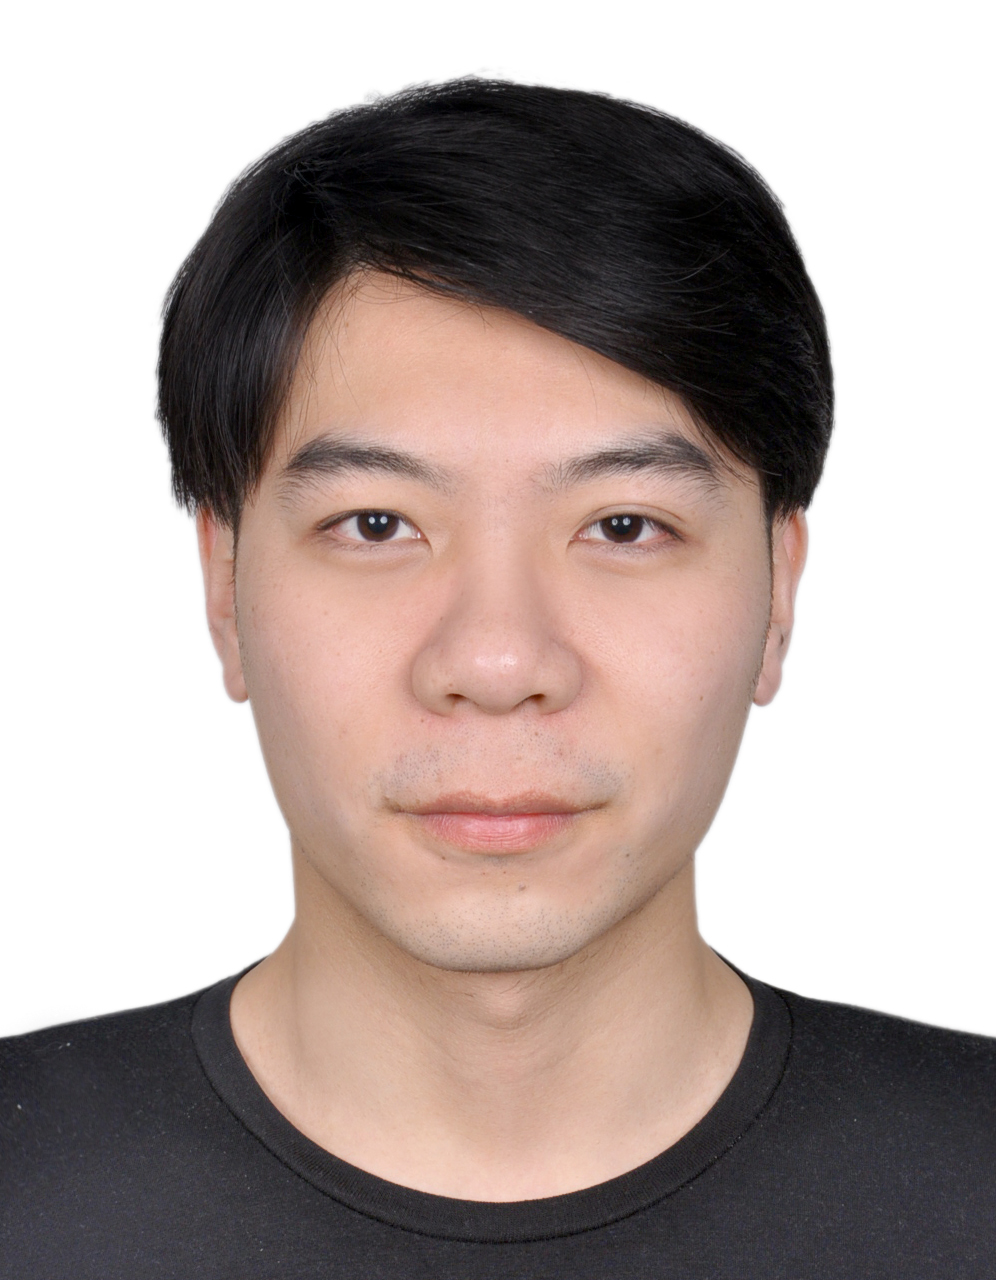
\includegraphics[height=3cm]{../people/binbinchen}
		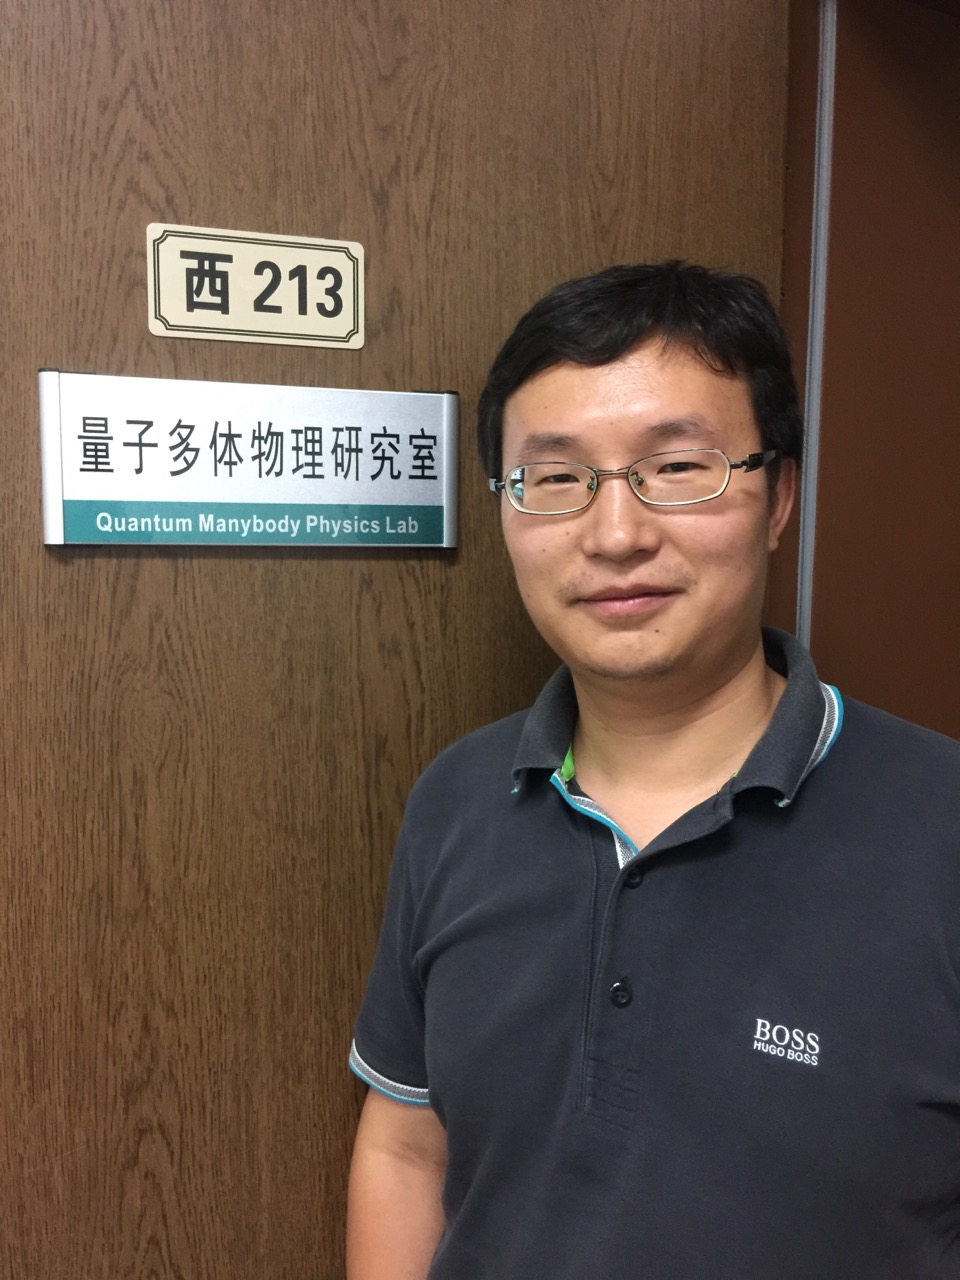
\includegraphics[height=3cm]{../people/weili}~~~~
		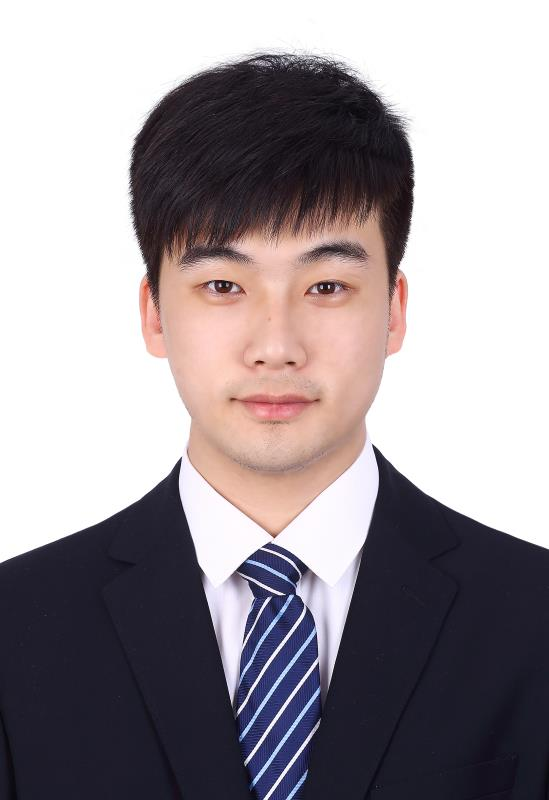
\includegraphics[height=3cm]{../people/xutaozeng}
		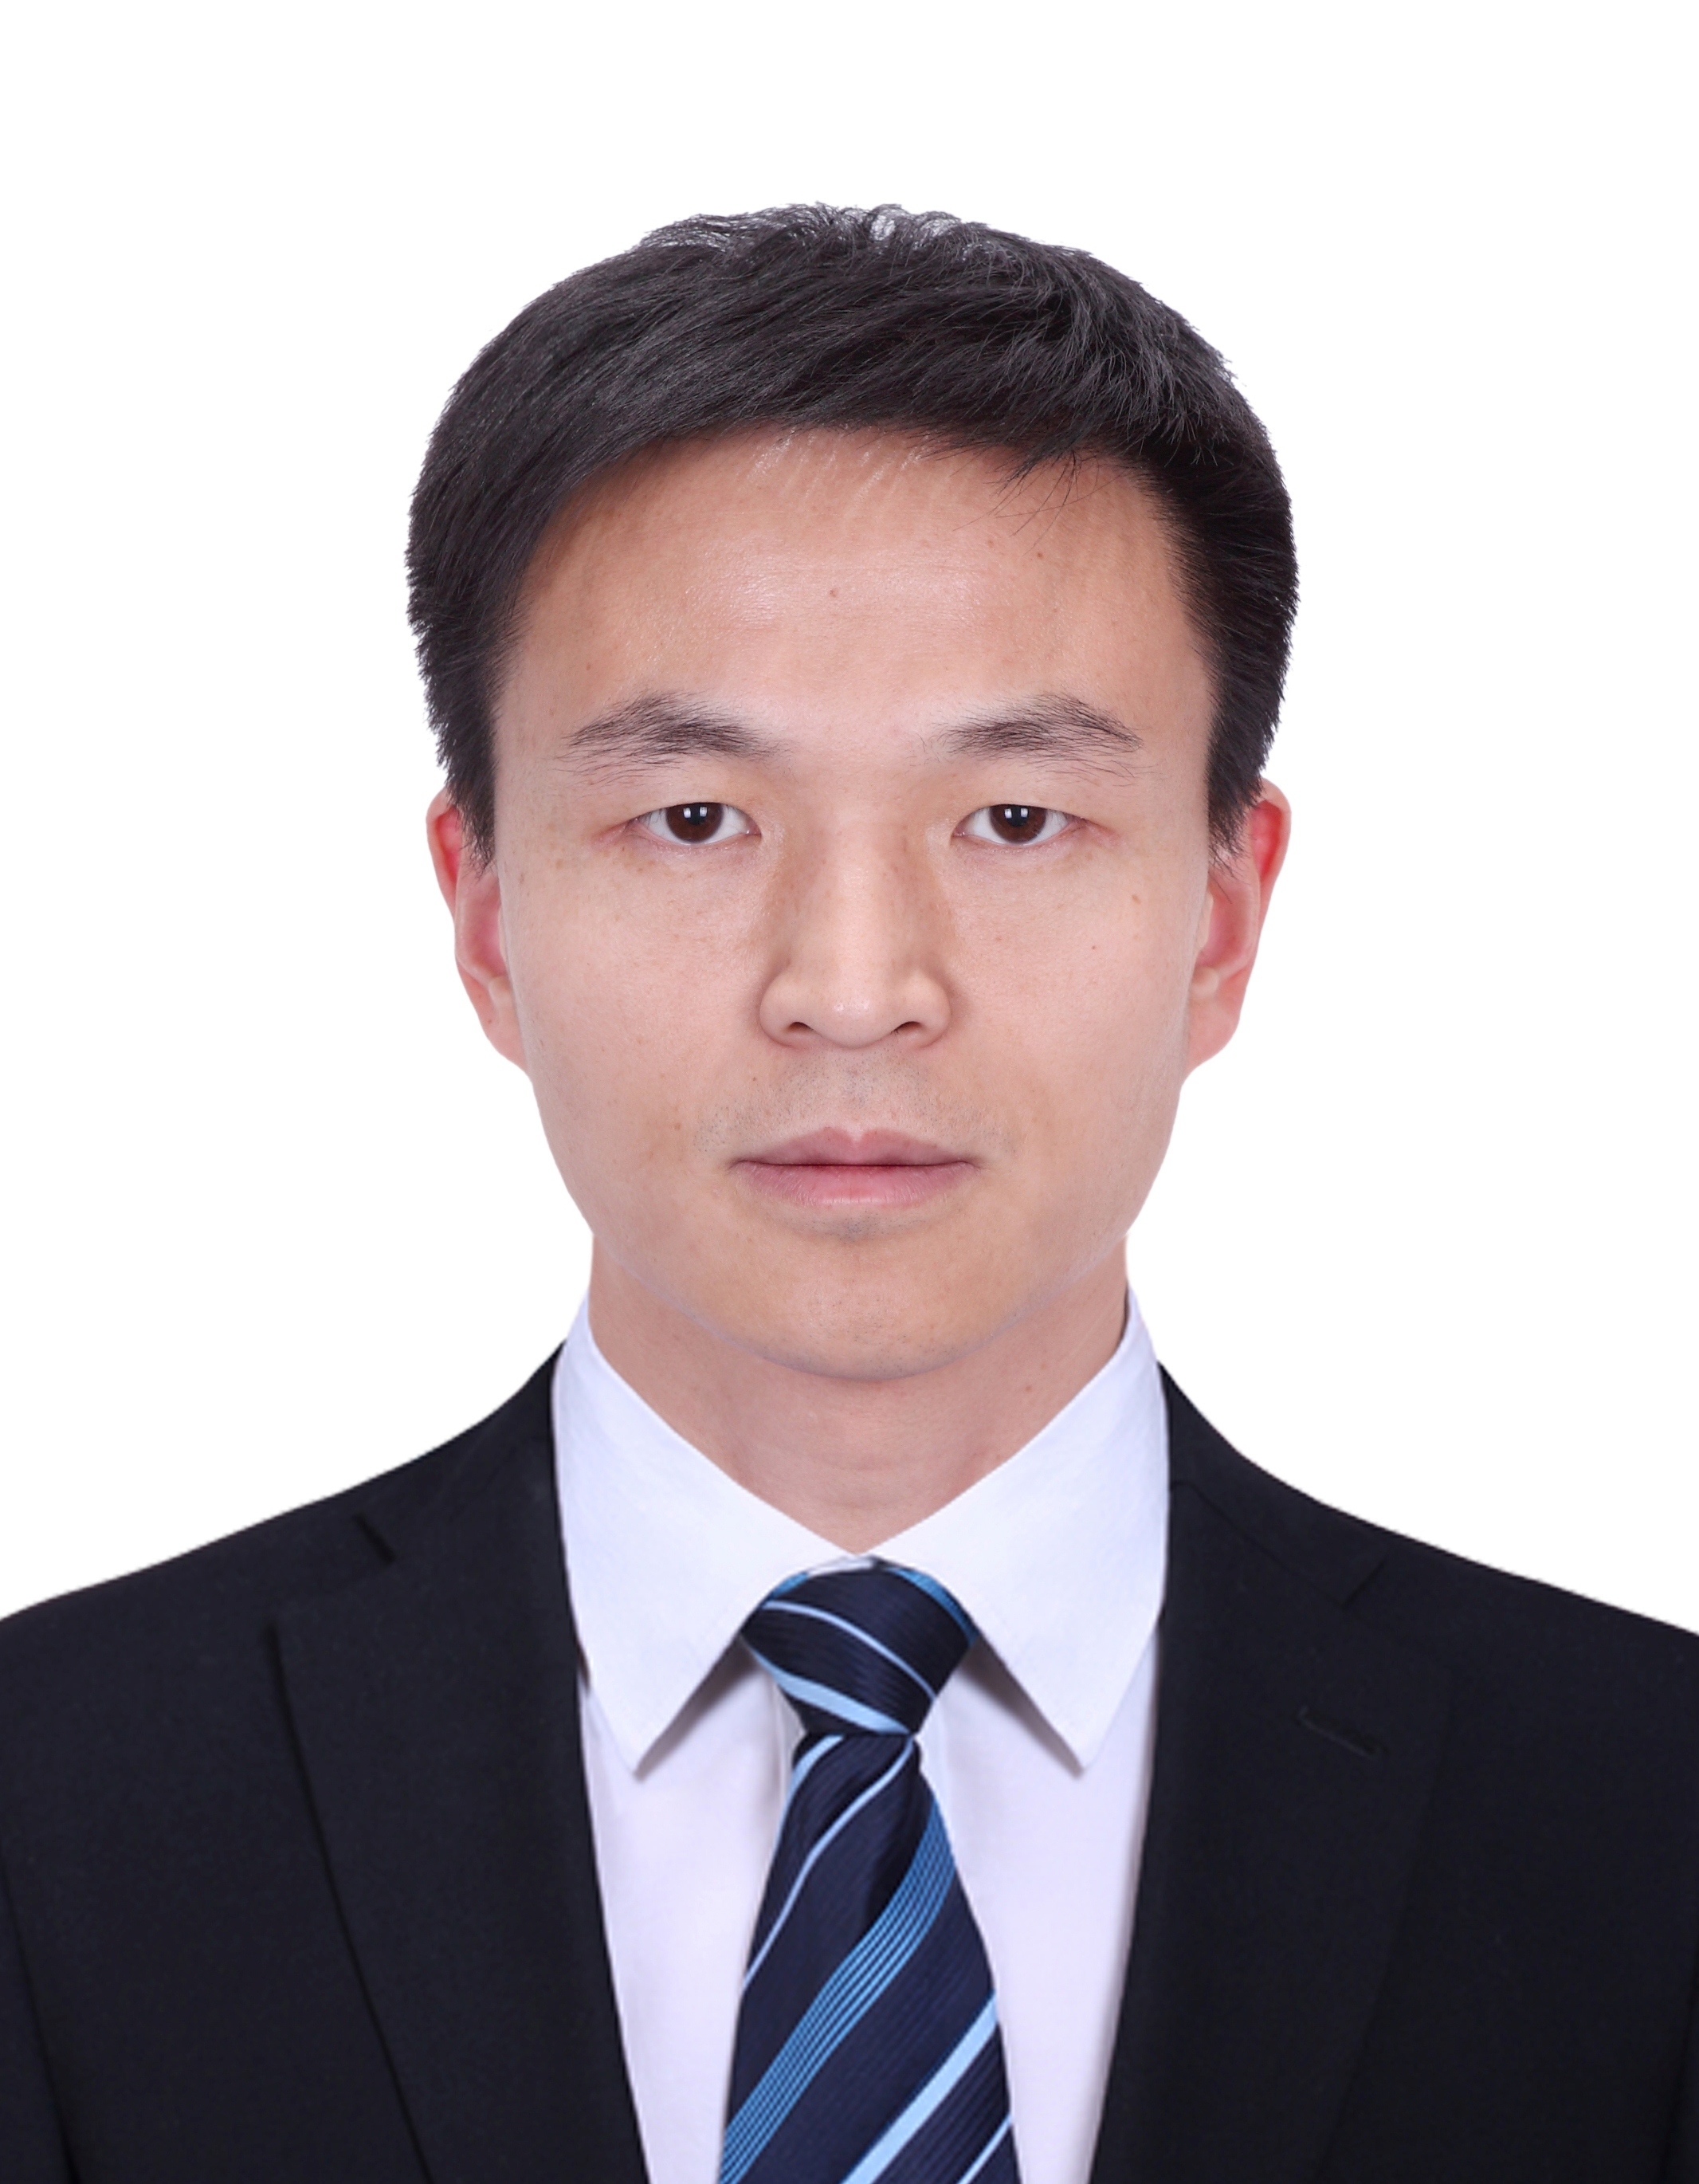
\includegraphics[height=3cm]{../people/xianleisheng}
	\end{center}
\end{frame}

\begin{frame}{Collaborators: Hong Kong University and Institute of Physics, CAS}
\begin{itemize}
	\item IOP, CAS: Yuan-Da Liao (廖元达).
	\item HKU: Zi Yang Meng (孟子杨).
	\item Quantum Monte Carlo simulations.
\end{itemize}
	\begin{center}
		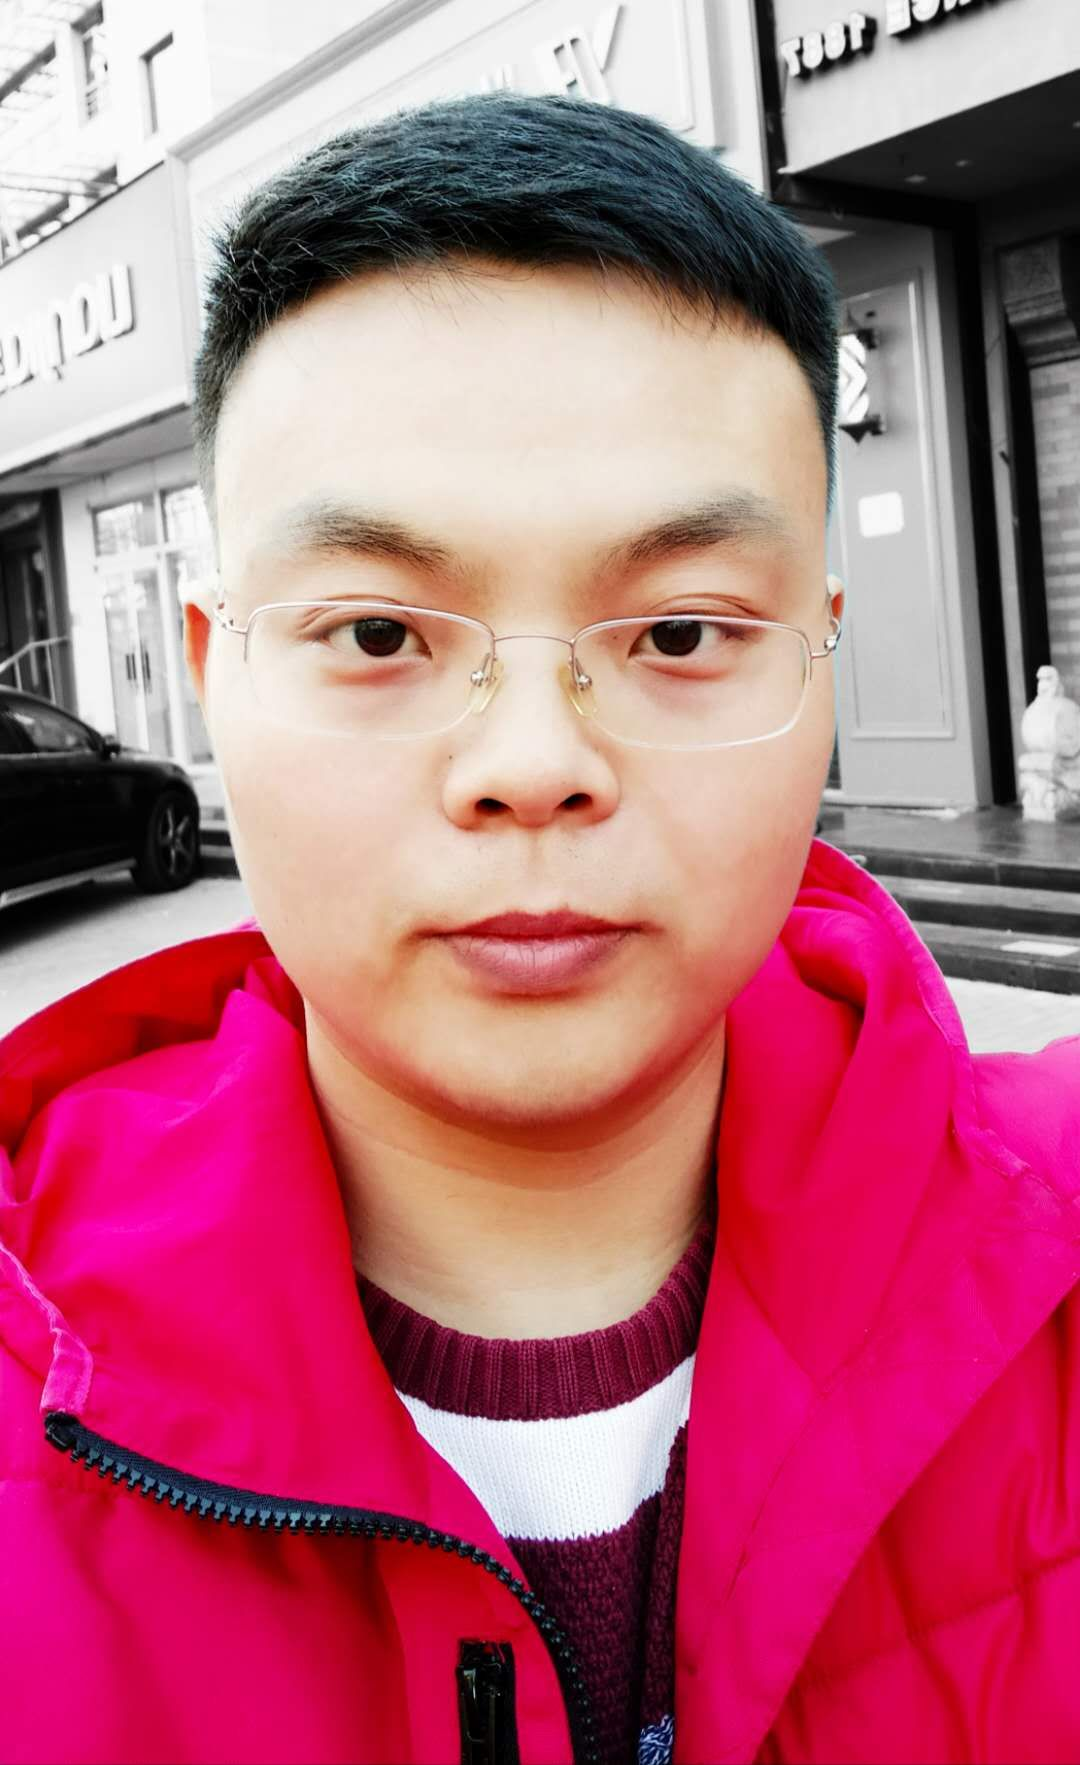
\includegraphics[height=3cm]{../people/yuandaliao}
		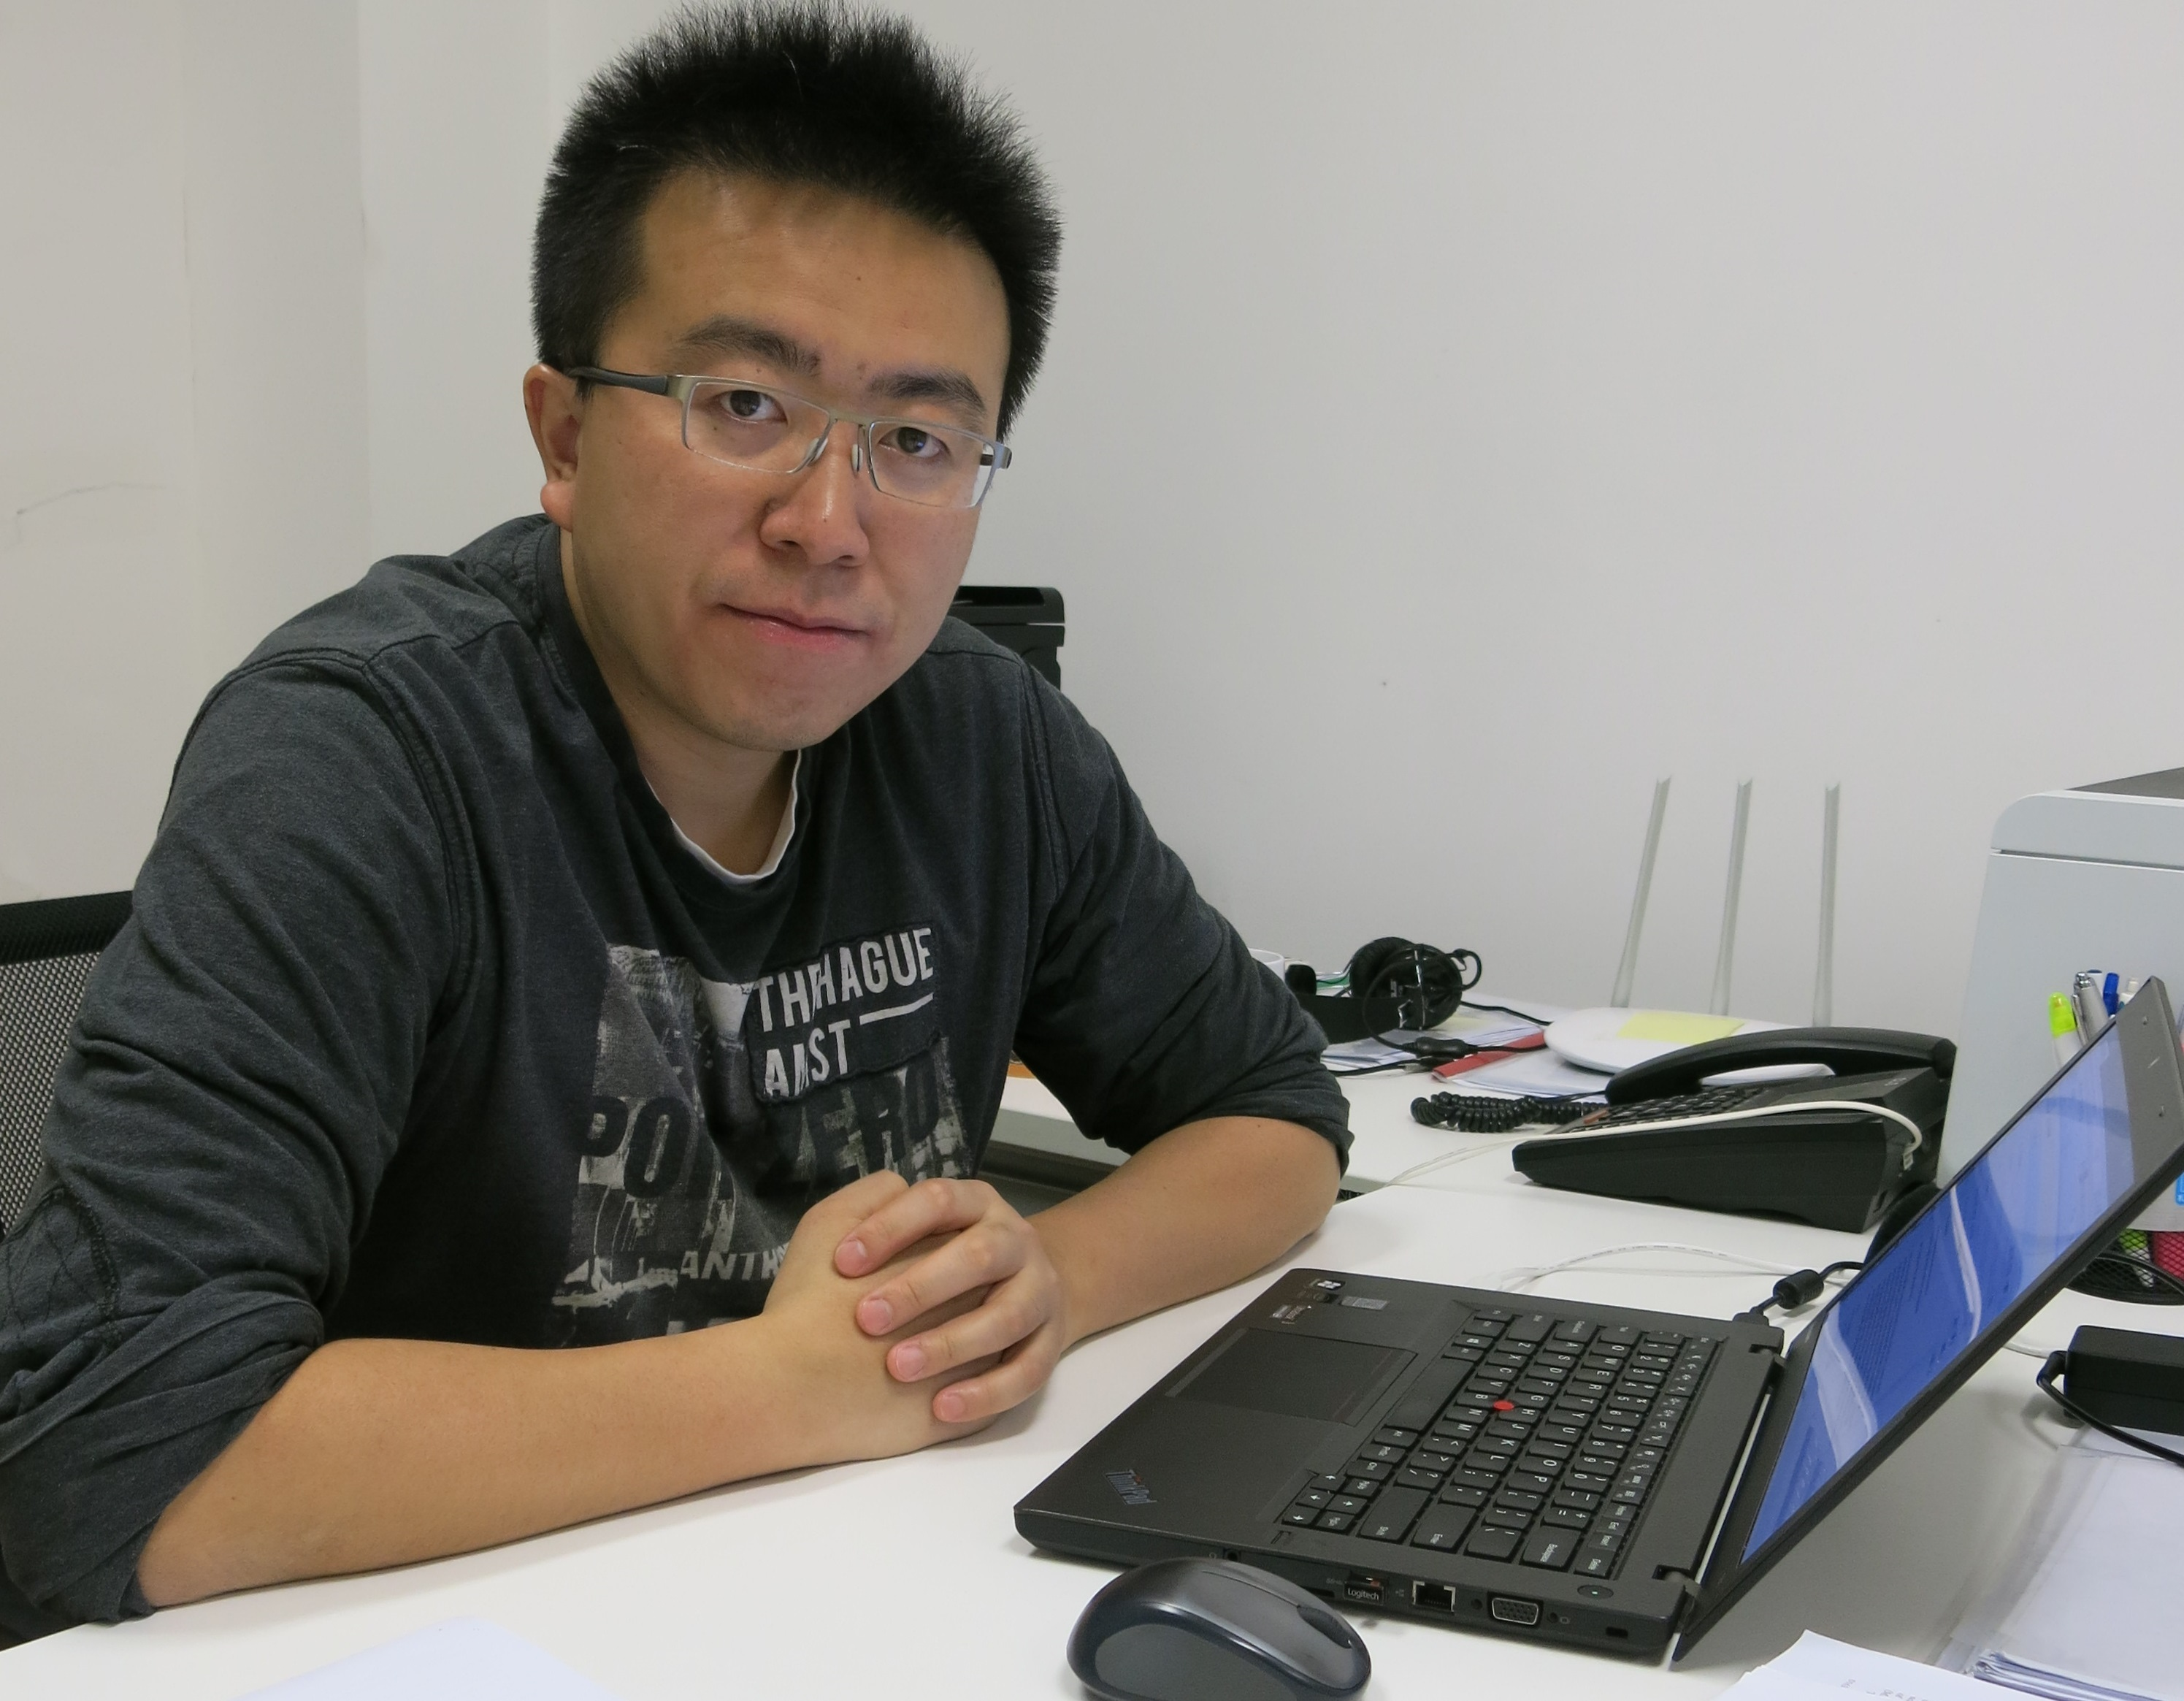
\includegraphics[height=3cm]{../people/ziyangmeng}
	\end{center}
\end{frame}

\begin{frame}{Collaborators: Nanjing University}
\begin{itemize}
	\item Zhen Ma (马祯), Yanyan Shangguan (上官艳艳), Zhentao Huang (黄振涛), Jinsheng Wen (温锦生).
	\item Single-crystal growth and susceptibility measurements.
\end{itemize}
	\begin{center}
		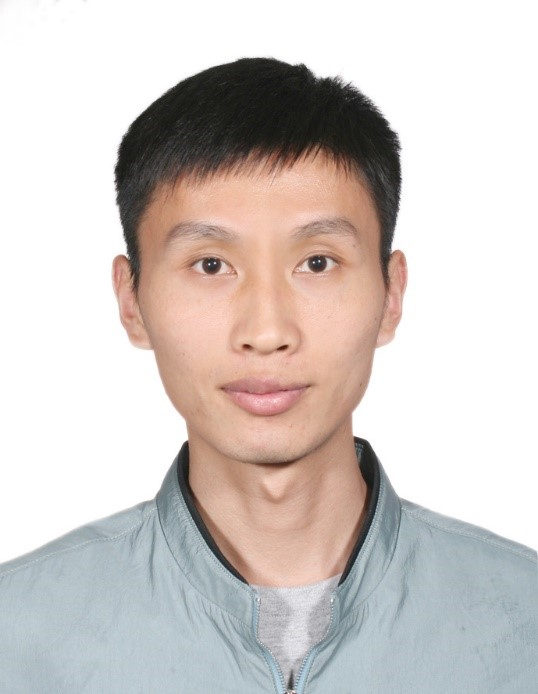
\includegraphics[height=3cm]{../people/zhenma}
		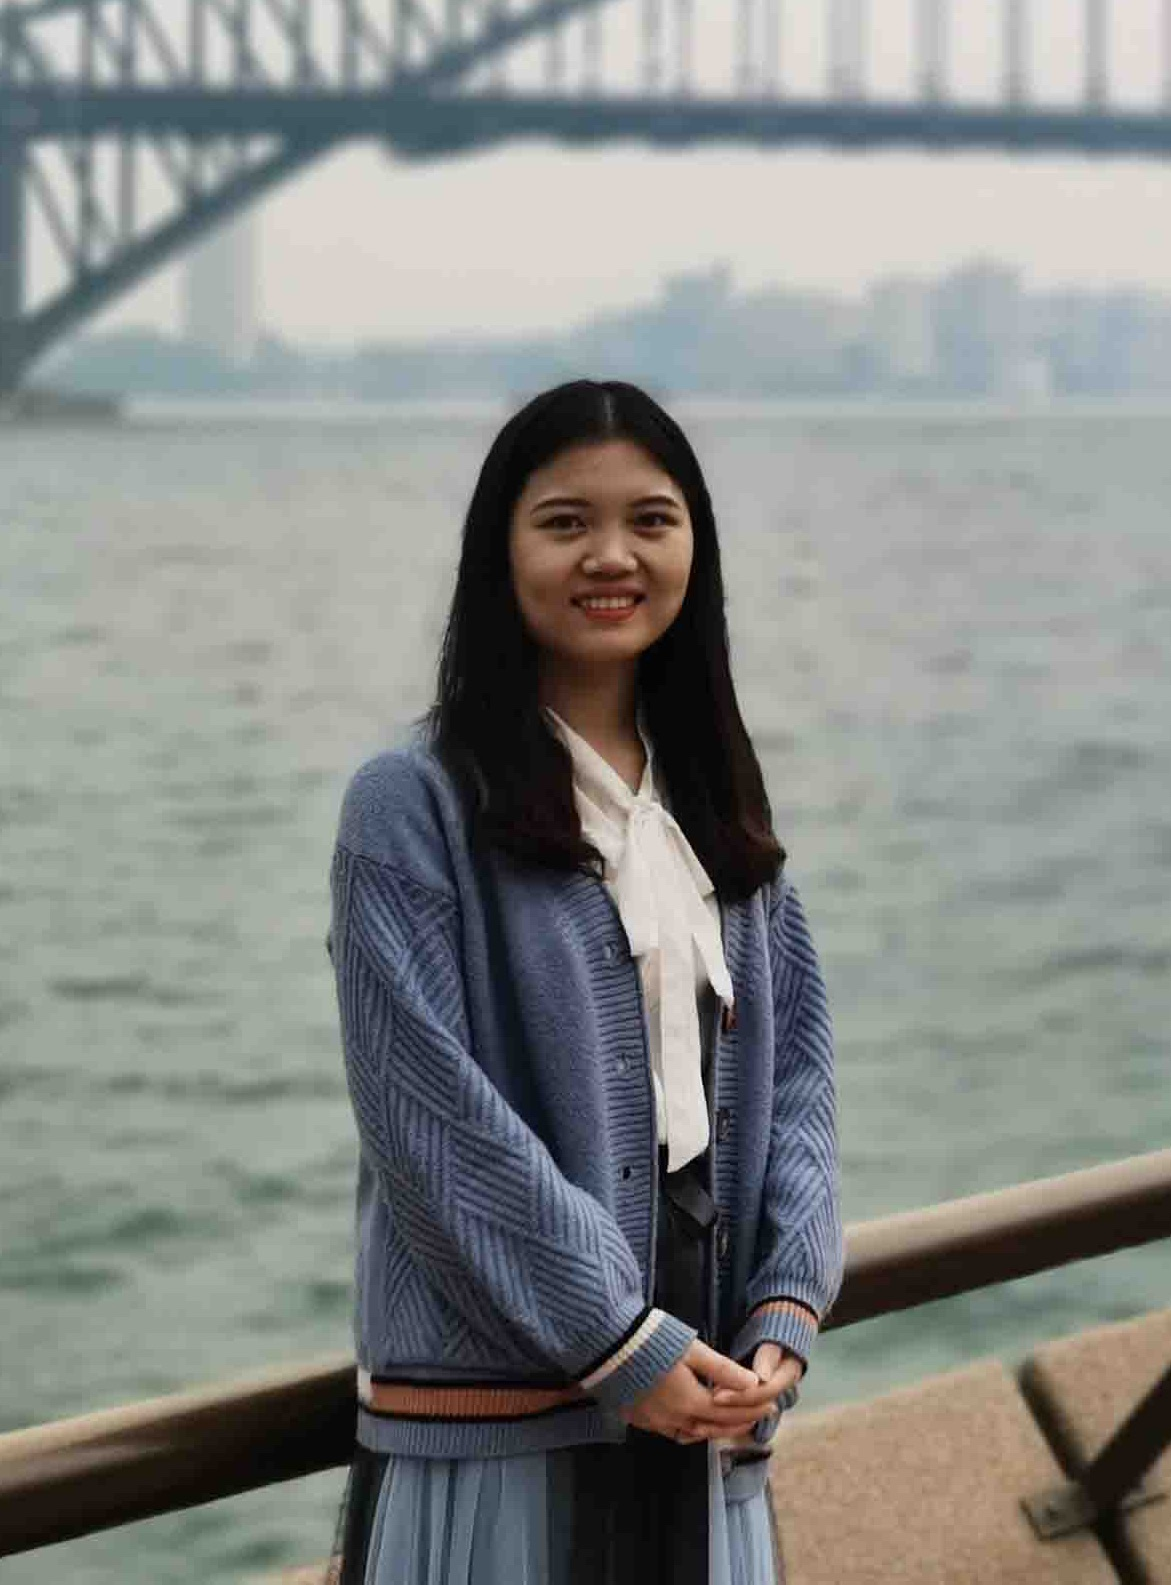
\includegraphics[height=3cm]{../people/yanyanshangguan}
		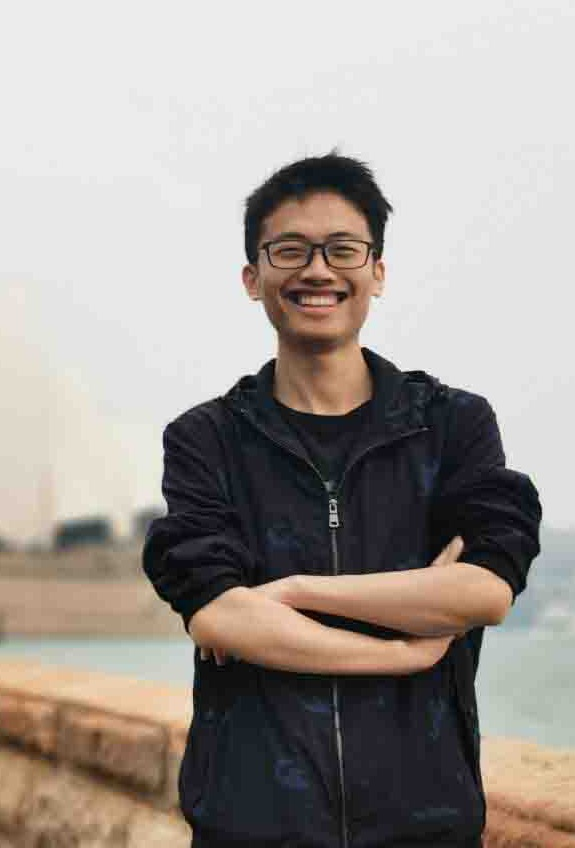
\includegraphics[height=3cm]{../people/zhentaohuang}
		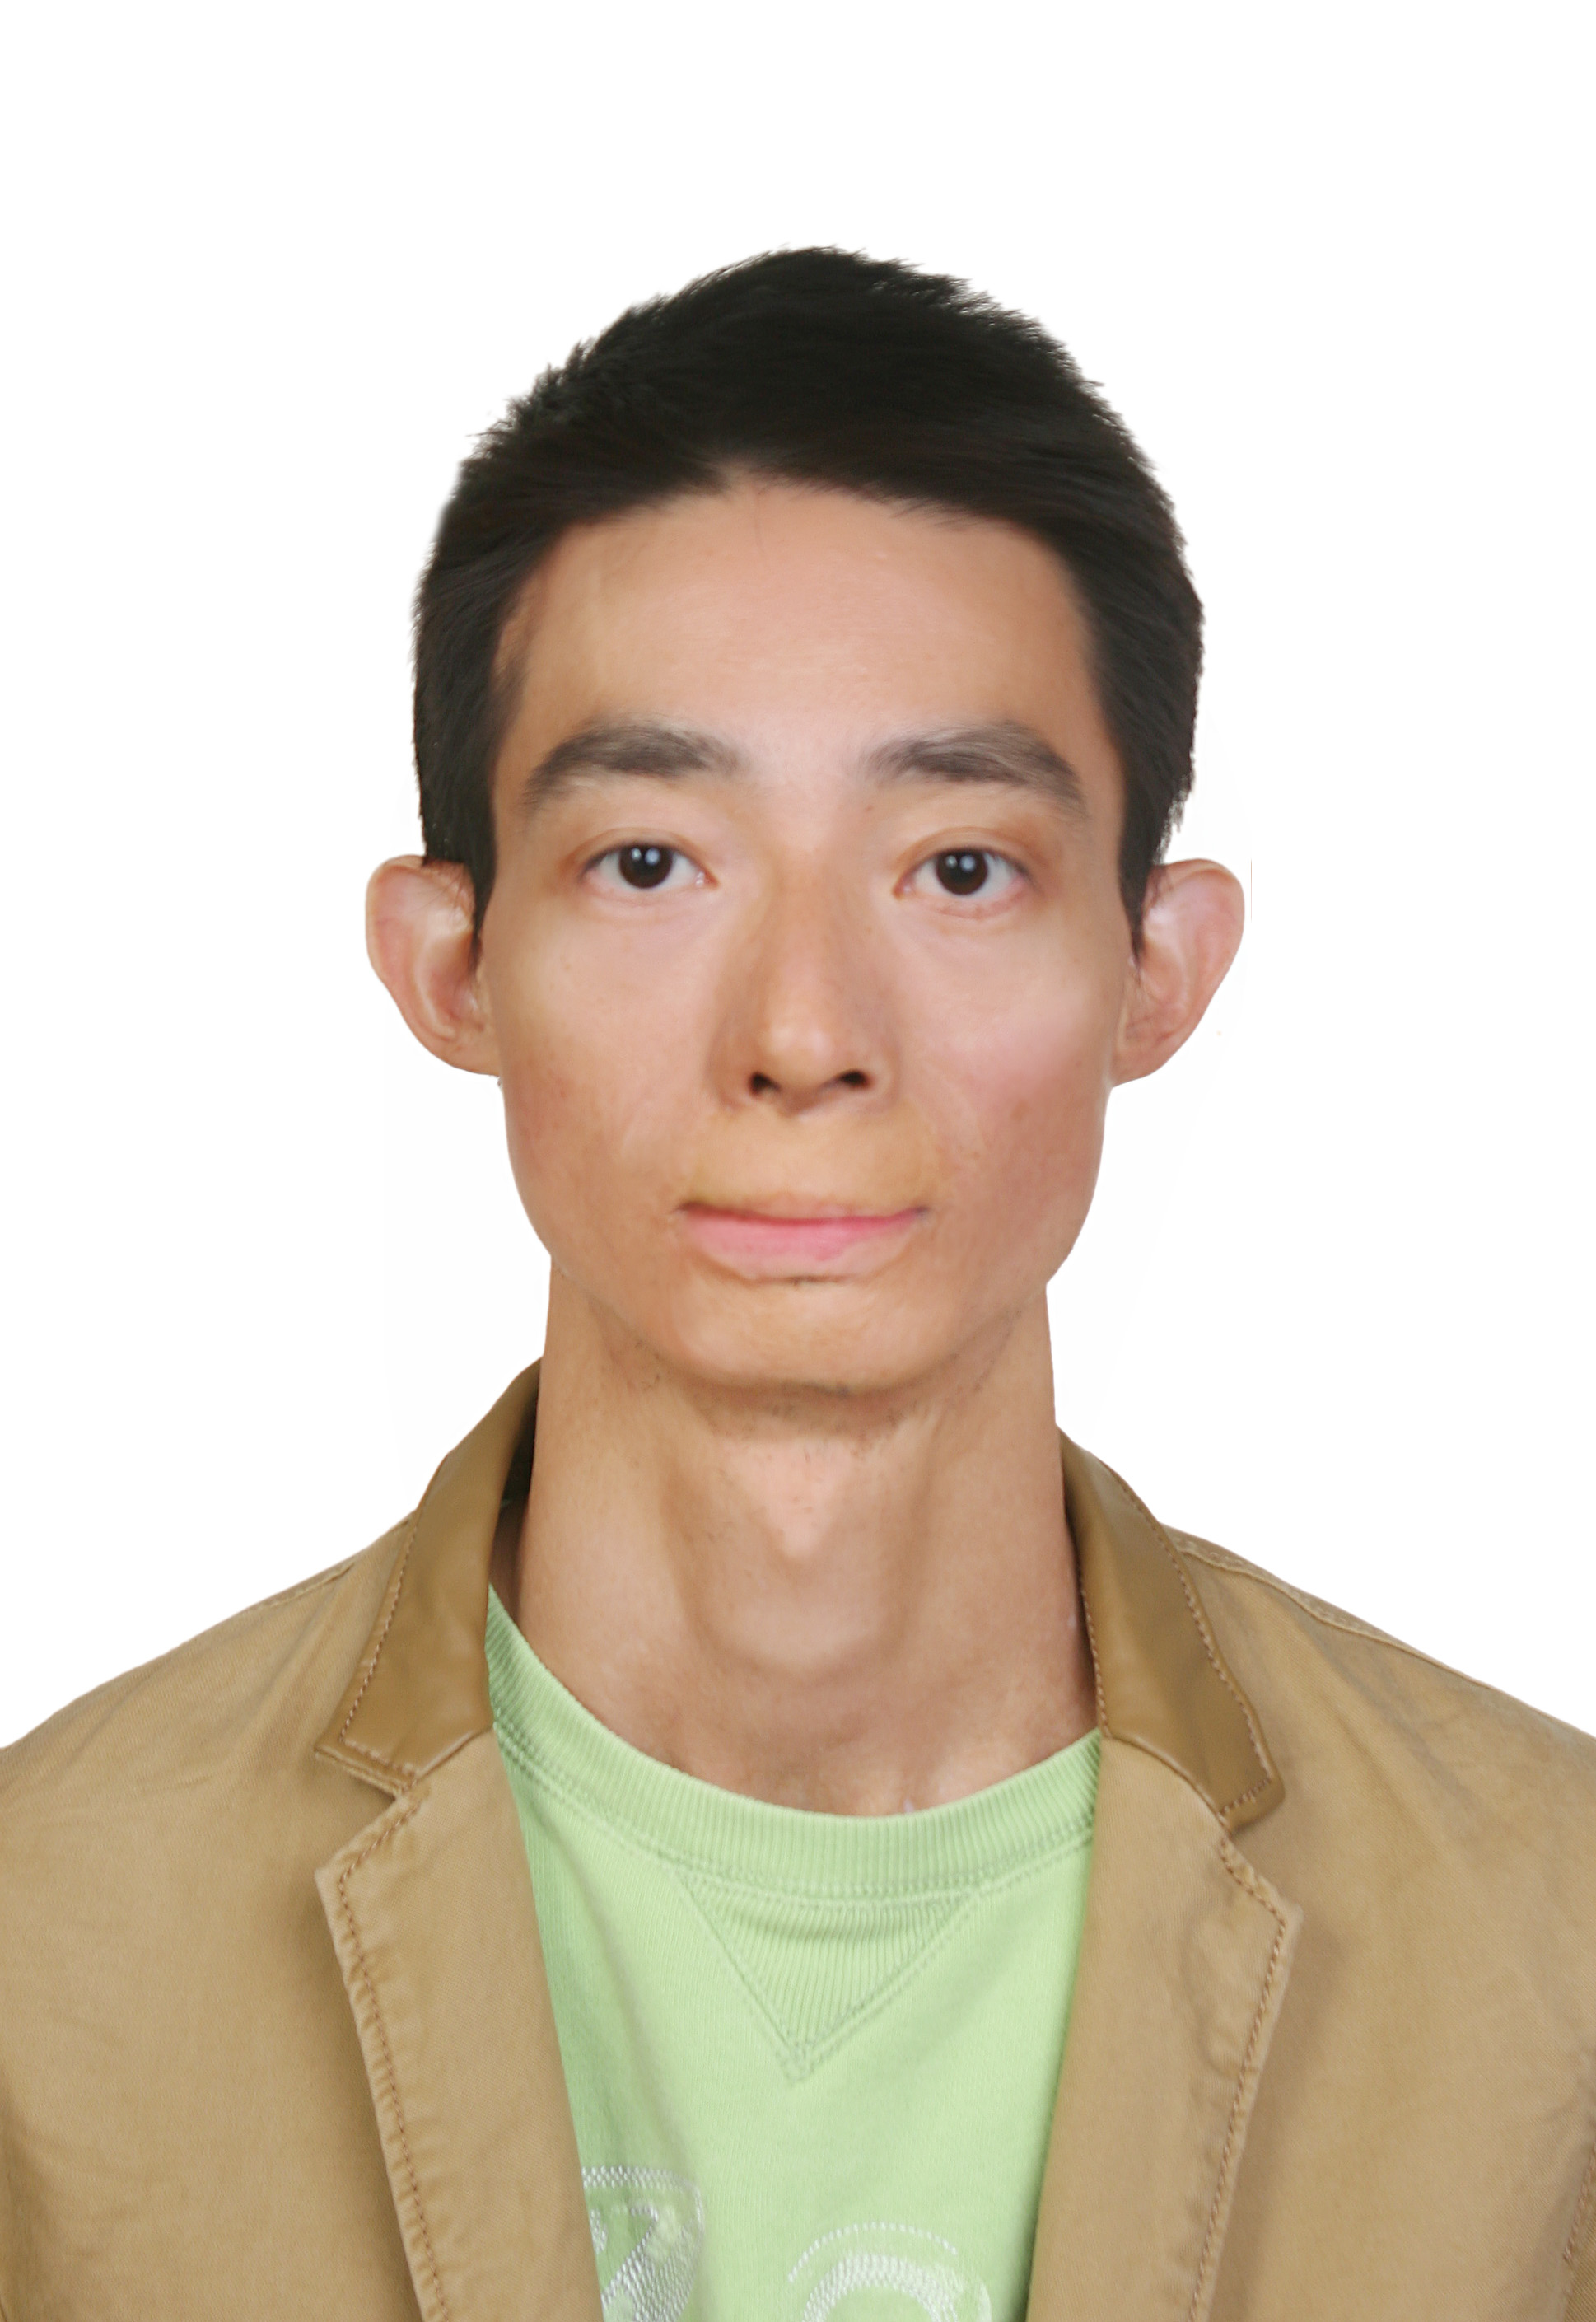
\includegraphics[height=3cm]{../people/jinshengwen}
	\end{center}
\end{frame}

\begin{frame}{Collaborators: Renmin University}
\begin{itemize}
	\item Ze Hu (胡泽), Chunsheng Ma (马春生), Yi Cui (崔祎), Weiqiang Yu (于伟强).
	\item NMR measurement and susceptibility measurements.
\end{itemize}
	\begin{center}
		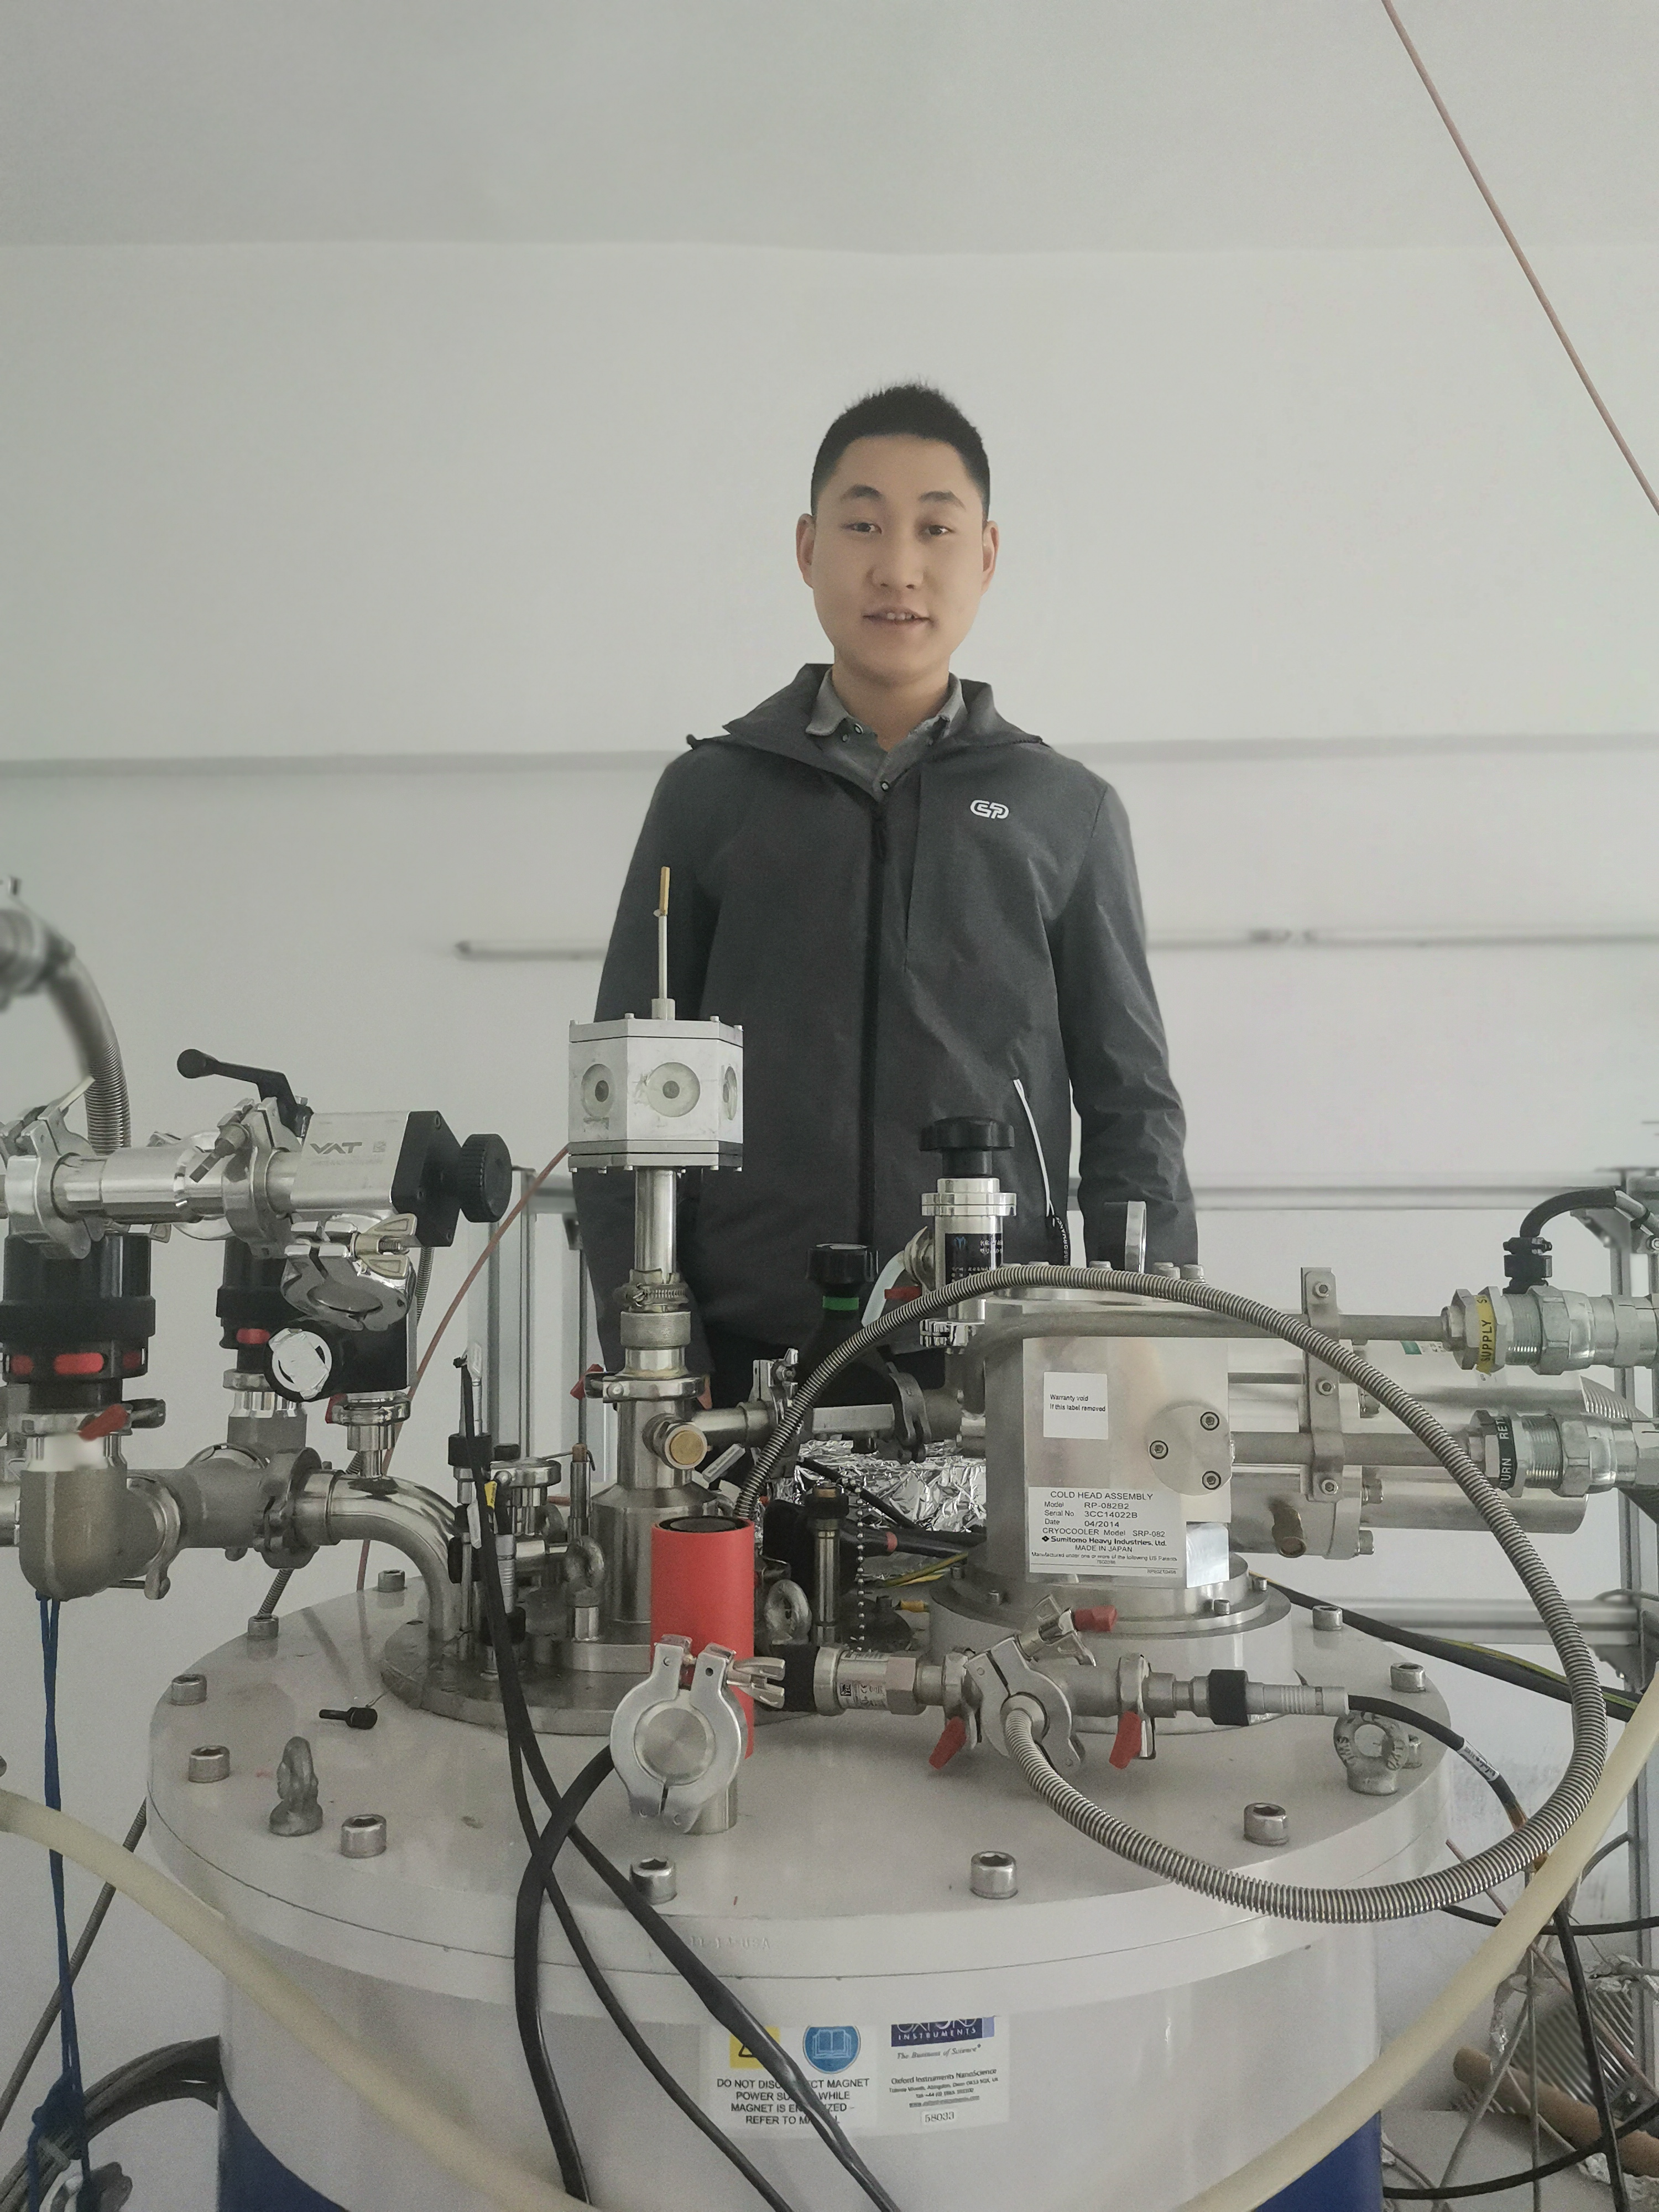
\includegraphics[height=5cm]{../people/zehu_large}
		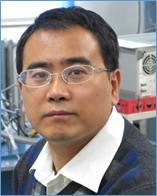
\includegraphics[height=3cm]{../people/weiqiangyu}
	\end{center}
\end{frame}

\begin{frame}{References}
\begin{itemize}
	\item Evidence of the Berezinskii-Kosterlitz-Thouless phase in a frustrated magnet\\
Ze Hu\#, Zhen Ma\#, Yuan-Da Liao\#, Han Li\#, Chunsheng Ma, Yi Cui, Yanyan Shangguan, Zhentao Huang, Yang Qi*, Wei Li*, Zi Yang Meng*, Jinsheng Wen*, and Weiqiang Yu*\\
Nature Communications \textbf{11} 5631 (2020).
	\item Kosterlitz-Thouless melting of magnetic order in the triangular quantum Ising material TmMgGaO${}_4$\\
Han Li\#, Yuan Da Liao\#, Bin-Bin Chen, Xu-Tao Zeng, Xian-Lei Sheng, Yang Qi*, Zi Yang Meng*, and Wei Li*\\
Nature Communications \textbf{11}, 1111 (2020)
\end{itemize}
\end{frame}

\begin{frame}{Outline}
	%\begin{columns}
	%\column{.7\textwidth}
		\tableofcontents
  %\end{columns}
  % You might wish to add the option [pausesections]
\end{frame}

\section{Introduction: Berezinskii-Kosterlitz-Thouless transition}

\begin{frame}
  \frametitle{Landau's paradigm: universality class and symmetry breaking}
  \begin{itemize}
  \item Phases are classified by symmetry breaking.
  \item Continuous phase transitions = spontaneous symmetry breaking.
  \item Universality class is determined by symmetry group and dimensionality.
  \end{itemize}
  \begin{center}
    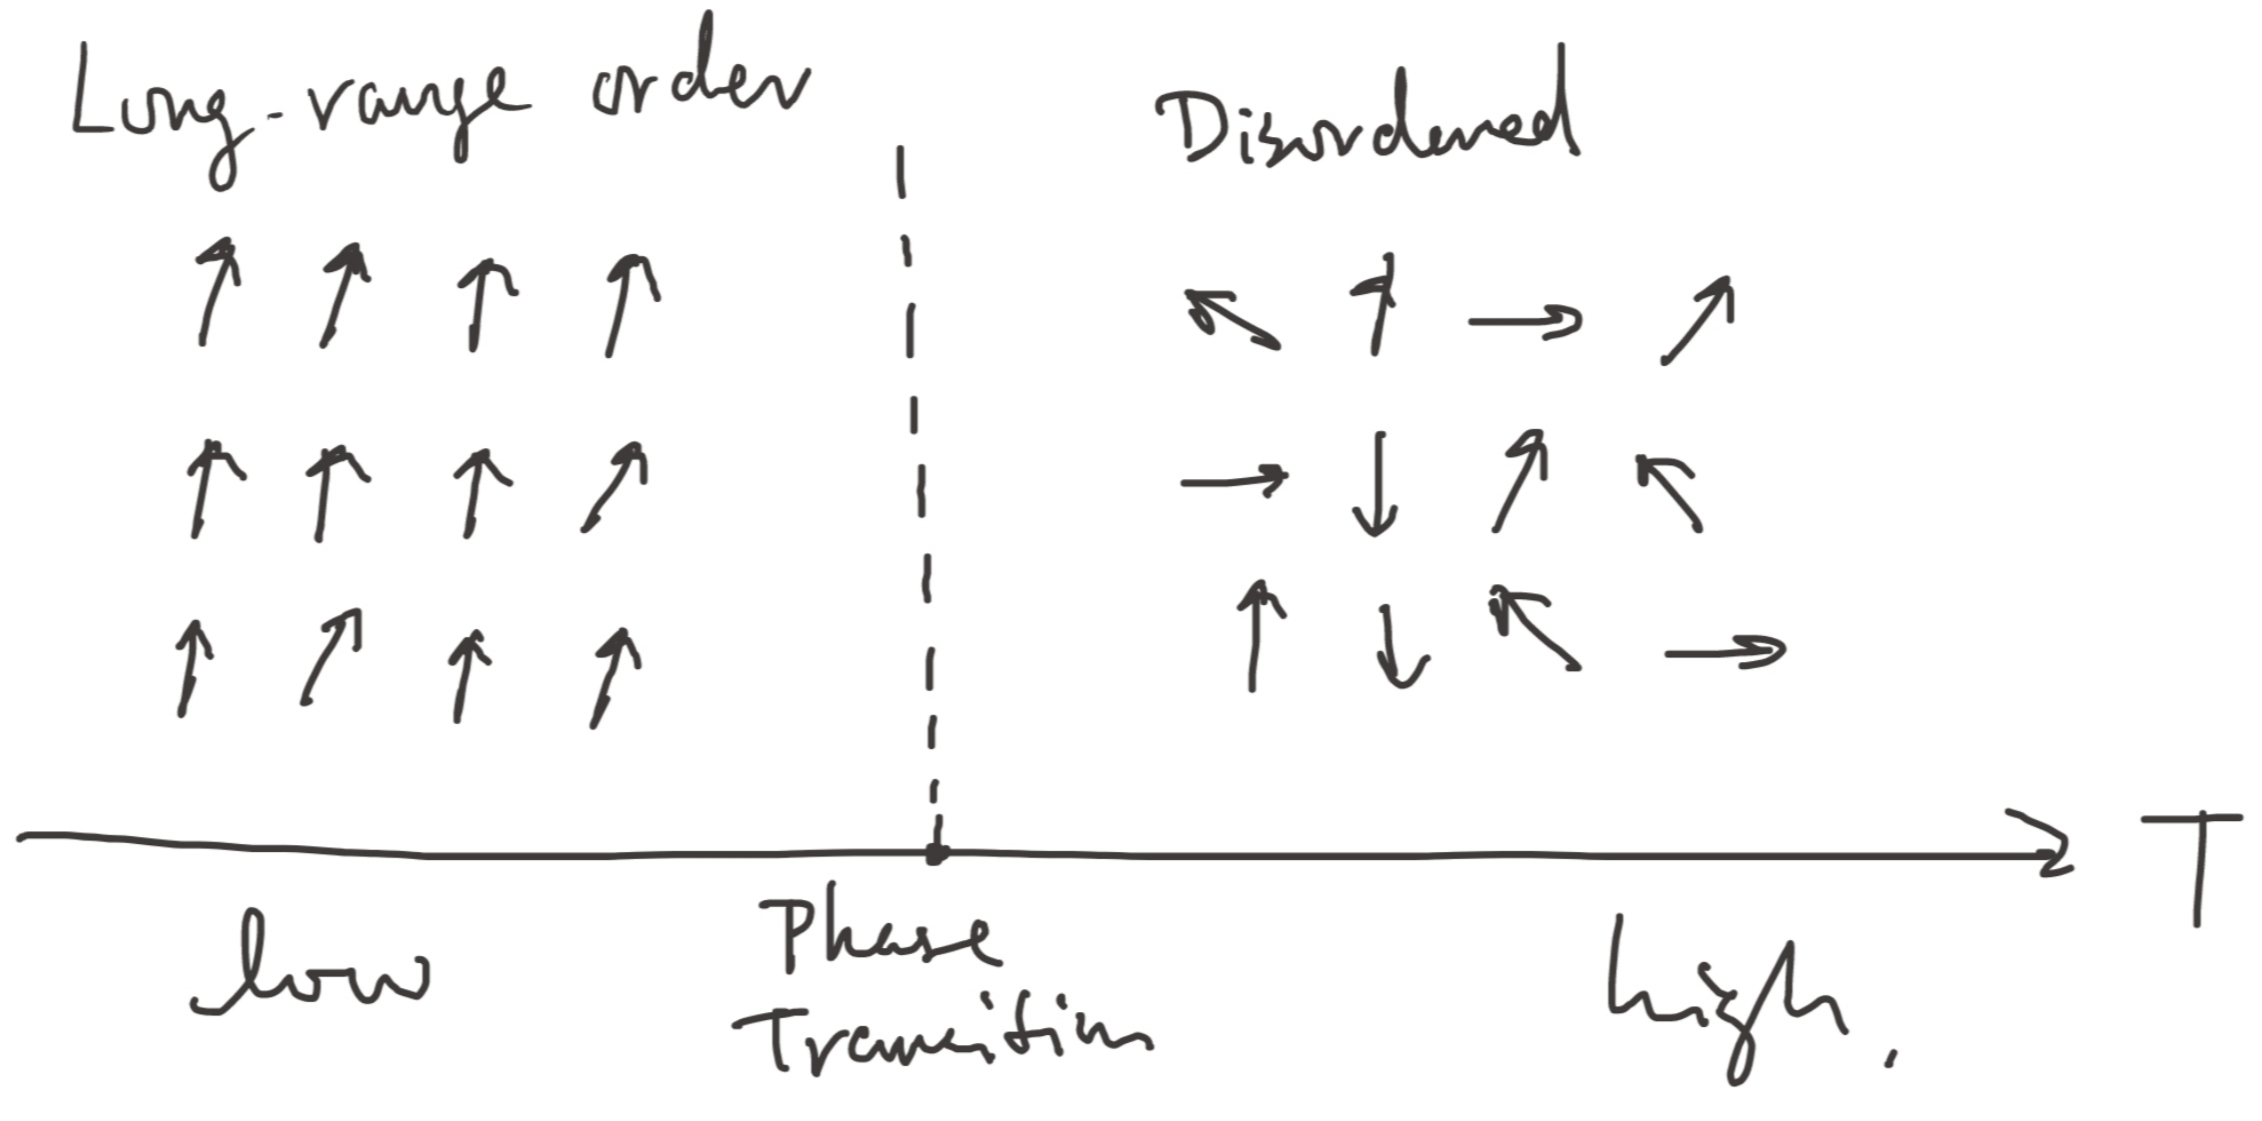
\includegraphics[height=5cm]{landau-paradigm}
  \end{center}
\end{frame}

\begin{frame}
  \frametitle{BKT transition: classical exception to Landau's paradigm}
  \begin{itemize}
  \item Mermin-Wagner Thm:\\a continuous symmetry cannot be broken at finite-$T$ in $D\leq2$.
  \item Exception: U(1) symmetry in 2D.
  \item Finite-$T$: a quasi-long-range order
    \[\langle \cos(\theta_i-\theta_j)\rangle\sim |i-j|^{-\eta},\quad \eta=\eta(T).\]
  \item BKT transition: QLR to disordered phase, caused by unbinding of vortex-antivortex pairs.
  \end{itemize}
  \begin{center}
    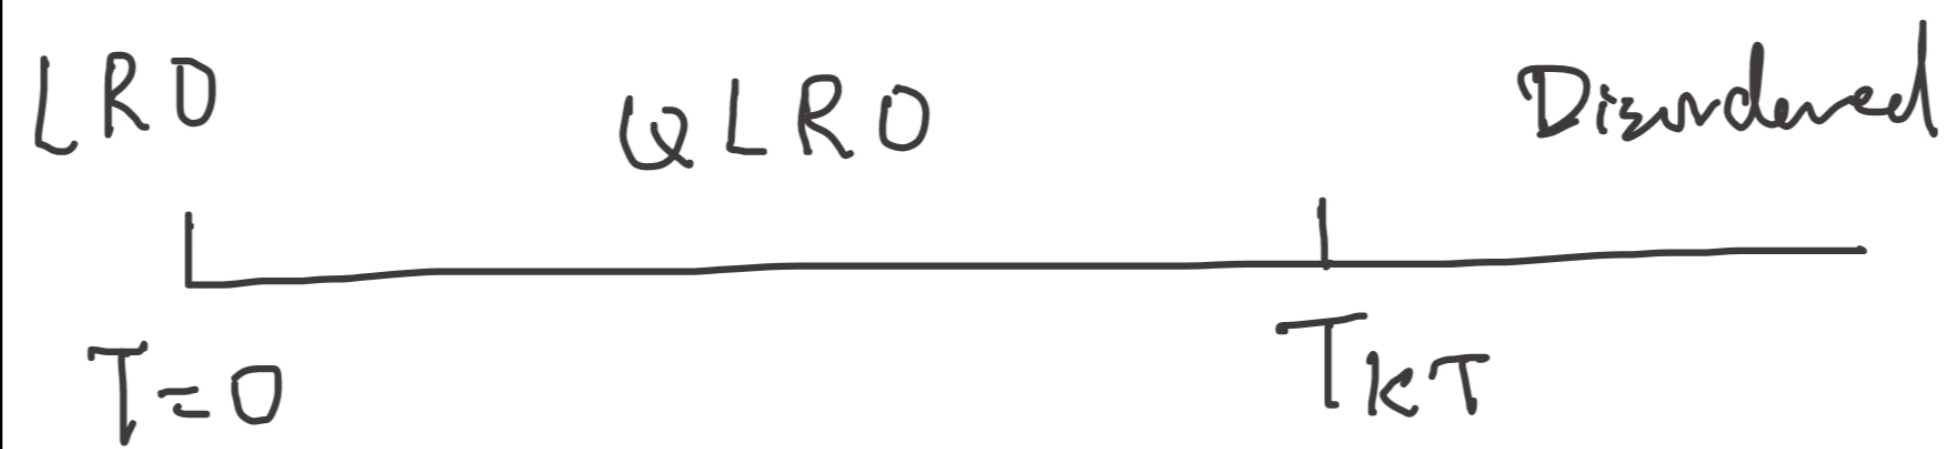
\includegraphics[width=.6\textwidth]{kt-pd}
  \end{center}
\end{frame}

\begin{frame}
  \frametitle{Realization of BKT transition}
  \begin{itemize}
  \item 2D superfluid (thin film).
  \item 2D superconductor (thin film).
  \item 2D ultracold bose gas.
  \item[?] Quantum magnets: 2D XY model?
    \[H=-J\sum_{\langle ij\rangle}\left(S_i^xS_j^x + S_i^yS_j^y\right).\]
  \end{itemize}
\end{frame}

\section{Material: From TmMgGaO${}_4$ to transverse-field Ising model}

\begin{frame}
  \frametitle{Effective DOF: Dipole-multipole doublet of Tm${}^{3+}$ ion}
  \begin{columns}
    \column{.6\textwidth}
    \begin{center}
      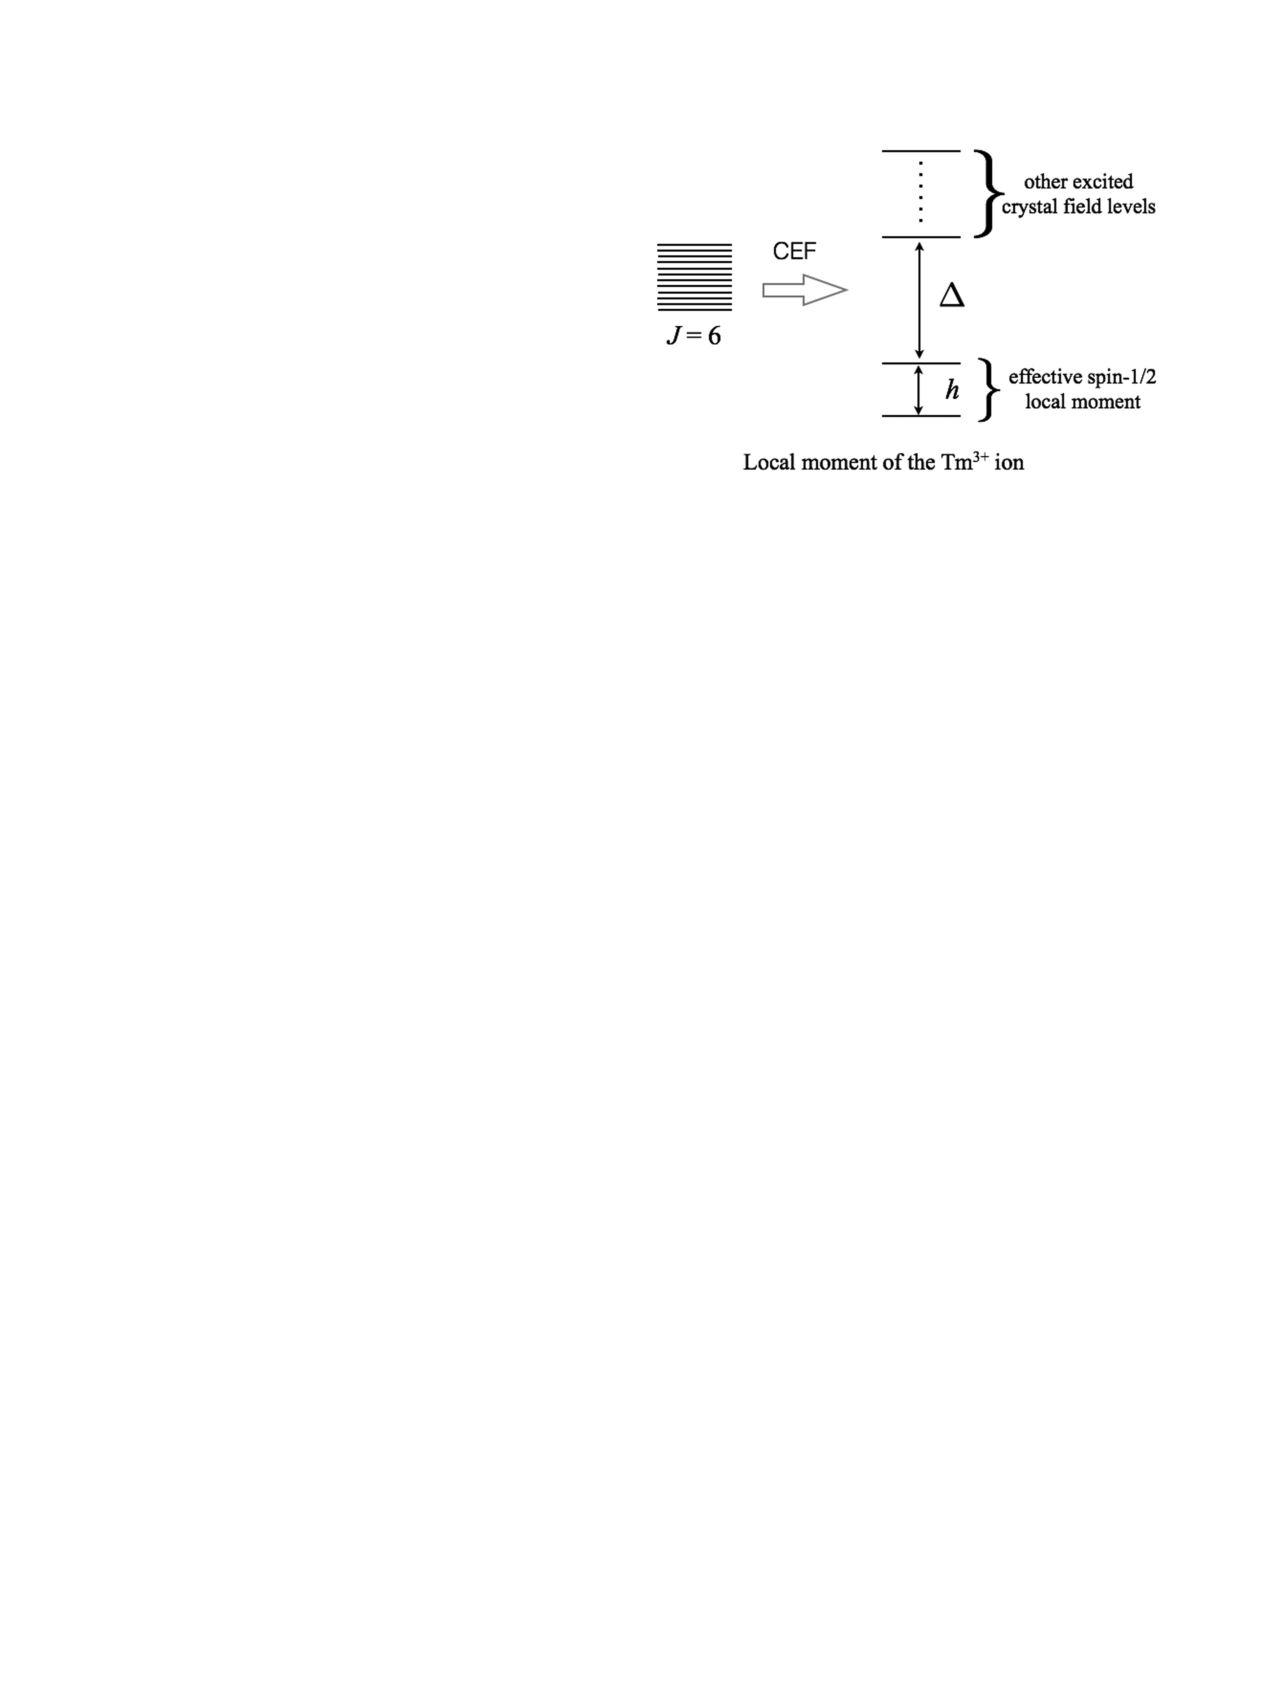
\includegraphics[width=\textwidth]{tm3+}

      {\small Changle Liu, Chun-Jiong Huang, and Gang Chen\\
        Phys. Rev. Research \textbf{2}, 043013 (2020).}
    \end{center}
    \column{.4\textwidth}
    \begin{itemize}
    \item Tm${}^{3+}$: $S=1$; no Kramers degeneracy.
    \item The two lowest levels of Tm${}^{3+}$ ion form an effective spin-$\frac12$.
    \item Dipole-multipole:
      \begin{align*}TS^{x,y}T^{-1}&=S^{x,y};\\
        TS^zT^{-1}&=-S^z.\end{align*}
    \item Splitting between two lowest levels: $H=-hS^x$.
    \end{itemize}
  \end{columns}
\end{frame}

\begin{frame}
  \frametitle{Effective model}
  \begin{itemize}
  \item Transverse-field Ising Model on a triangular lattice.
  \item Antiferromagnetic interaction: fully frustrated.
  \item $h$ is the CEF splitting between two levels, not the actual magnetif field.
  \item $h^z$ couples to $S_i^z$.
  \end{itemize}
  \[H = J_1\sum_{\langle ij\rangle}S_i^zS_j^z +J_2\sum_{\langle\langle ij\rangle\rangle}S_i^zS_j^z - \sum_i\left(hS_i^x + h^zS_i^z\right). \]

  \begin{center}
    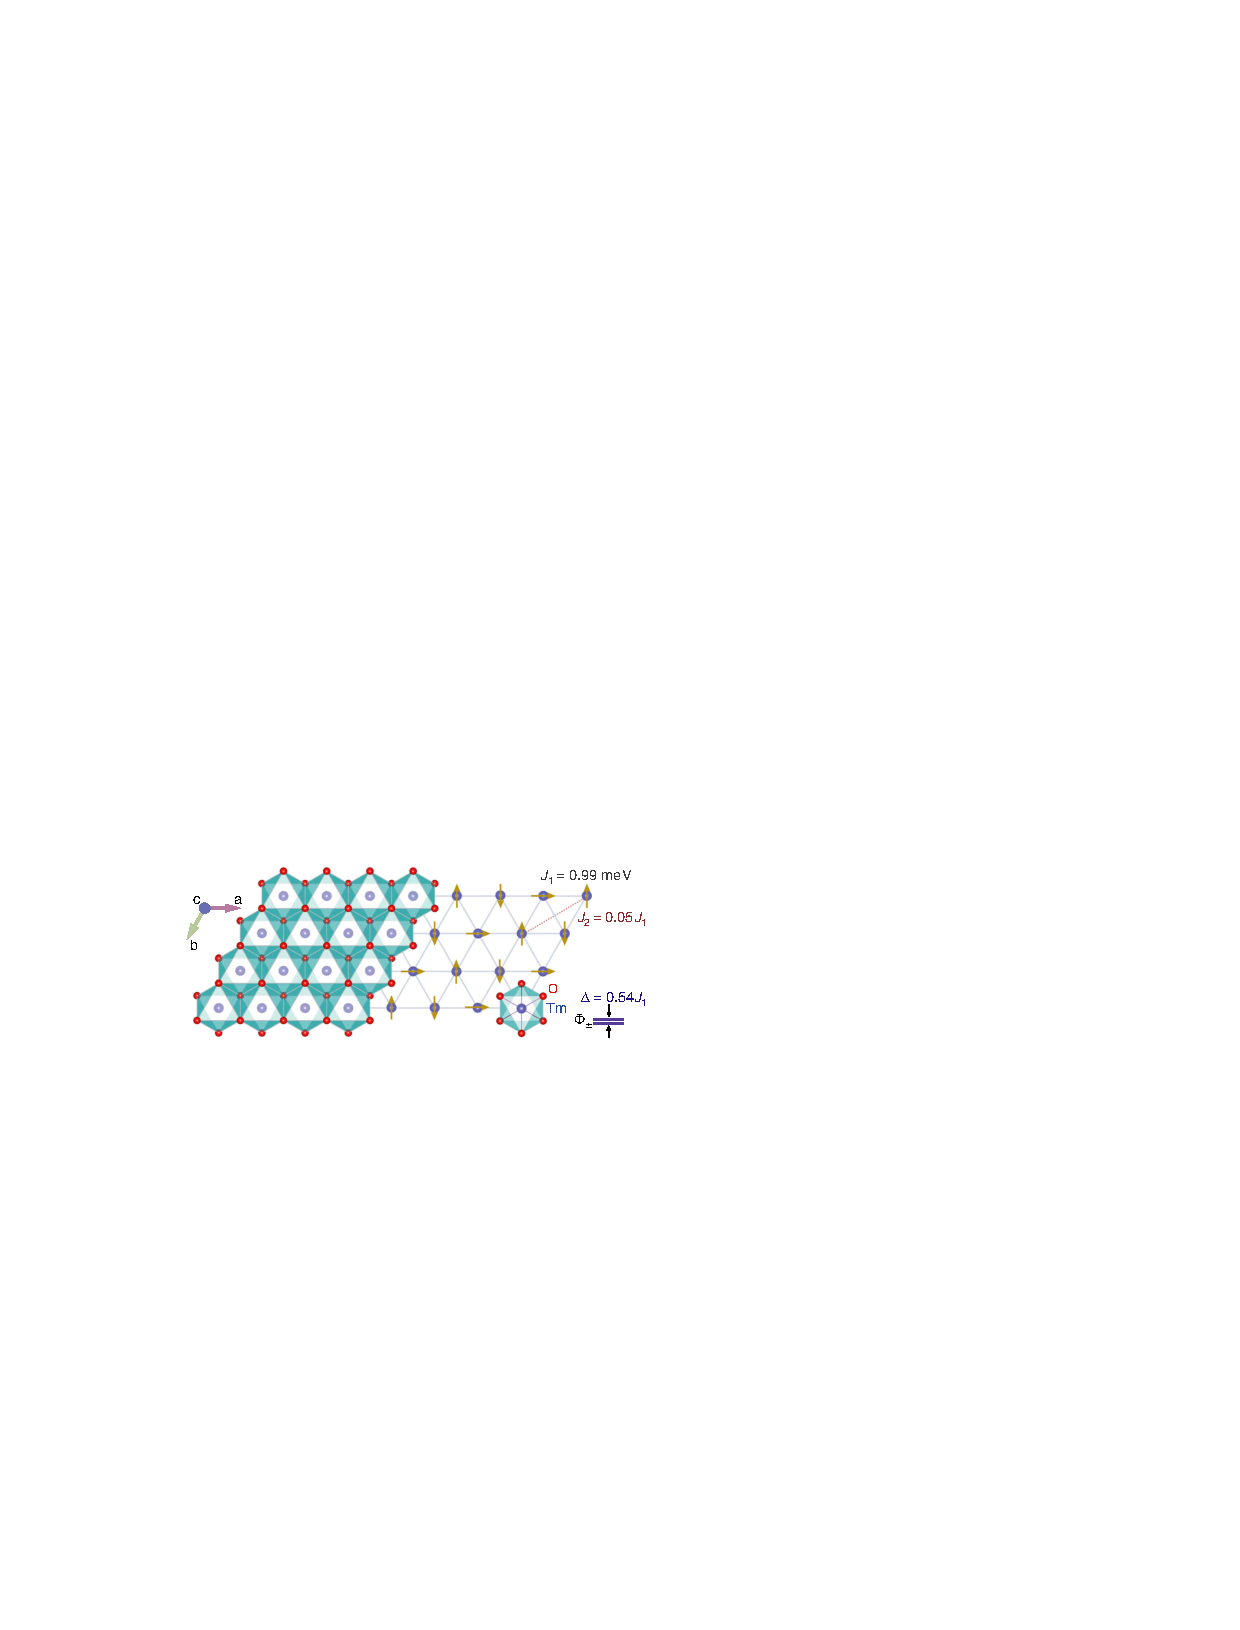
\includegraphics{lattice-afm}
  \end{center}
  \emph{\small Such a model was first introduced in Yao Shen, Changle Liu, ......, Gang Chen \& Jun Zhao, Nat. Comm. \textbf{10}, 4530 (2019).}
\end{frame}

\begin{frame}
  \frametitle{Numerically determination of the model}
  \begin{itemize}
    \item<1-> We use two numerical methods to solve the model,
    \begin{enumerate}
      \item<2-> XTRG = eXponential Tensor Renormalization Group.\\
      B-B Chen et al, Phys. Rev. X \textbf{8}, 031082 (2018).
      \item<3-> QMC = Quantum Monte Carlo: the model is sign-problem free.
      \item<4-> SAC = Stochastic Analytic Continuation.\\
      A W Sandvik, Phys. Rev. E \textbf{94}, 063308 (2016).
    \end{enumerate}
    \item<5-> The numerical results is compared to experiments to find best parameters.
    %\item Model parameters are determined by looking for a best fit.
    \item<6-> XTRG: provides a quick comparison between different model parameters.
    \item<6-> QMC: for benchmarking XTRG and extracting spin spectrum using SAC.
  \end{itemize}

  \begin{center}
    \visible<2->{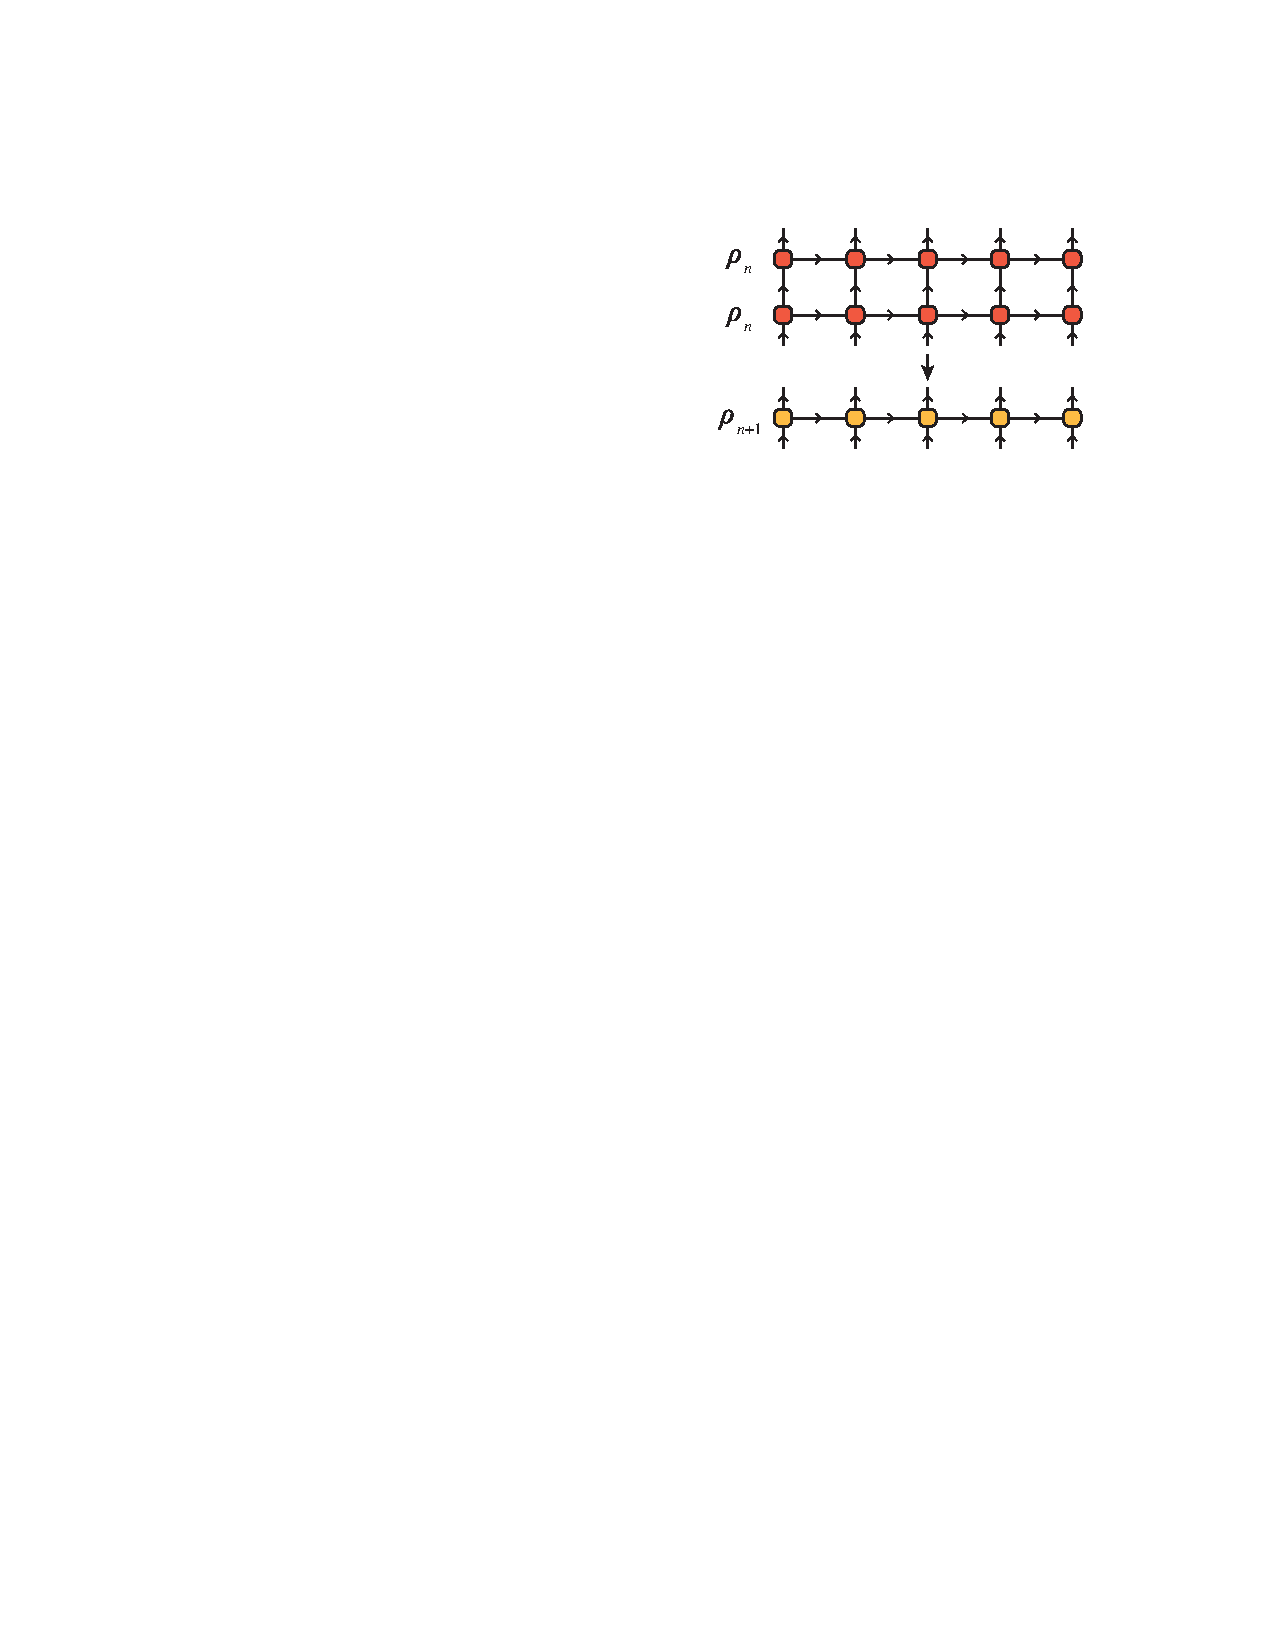
\includegraphics[height=3cm]{xtrg2}}~~~~~~
    \visible<4->{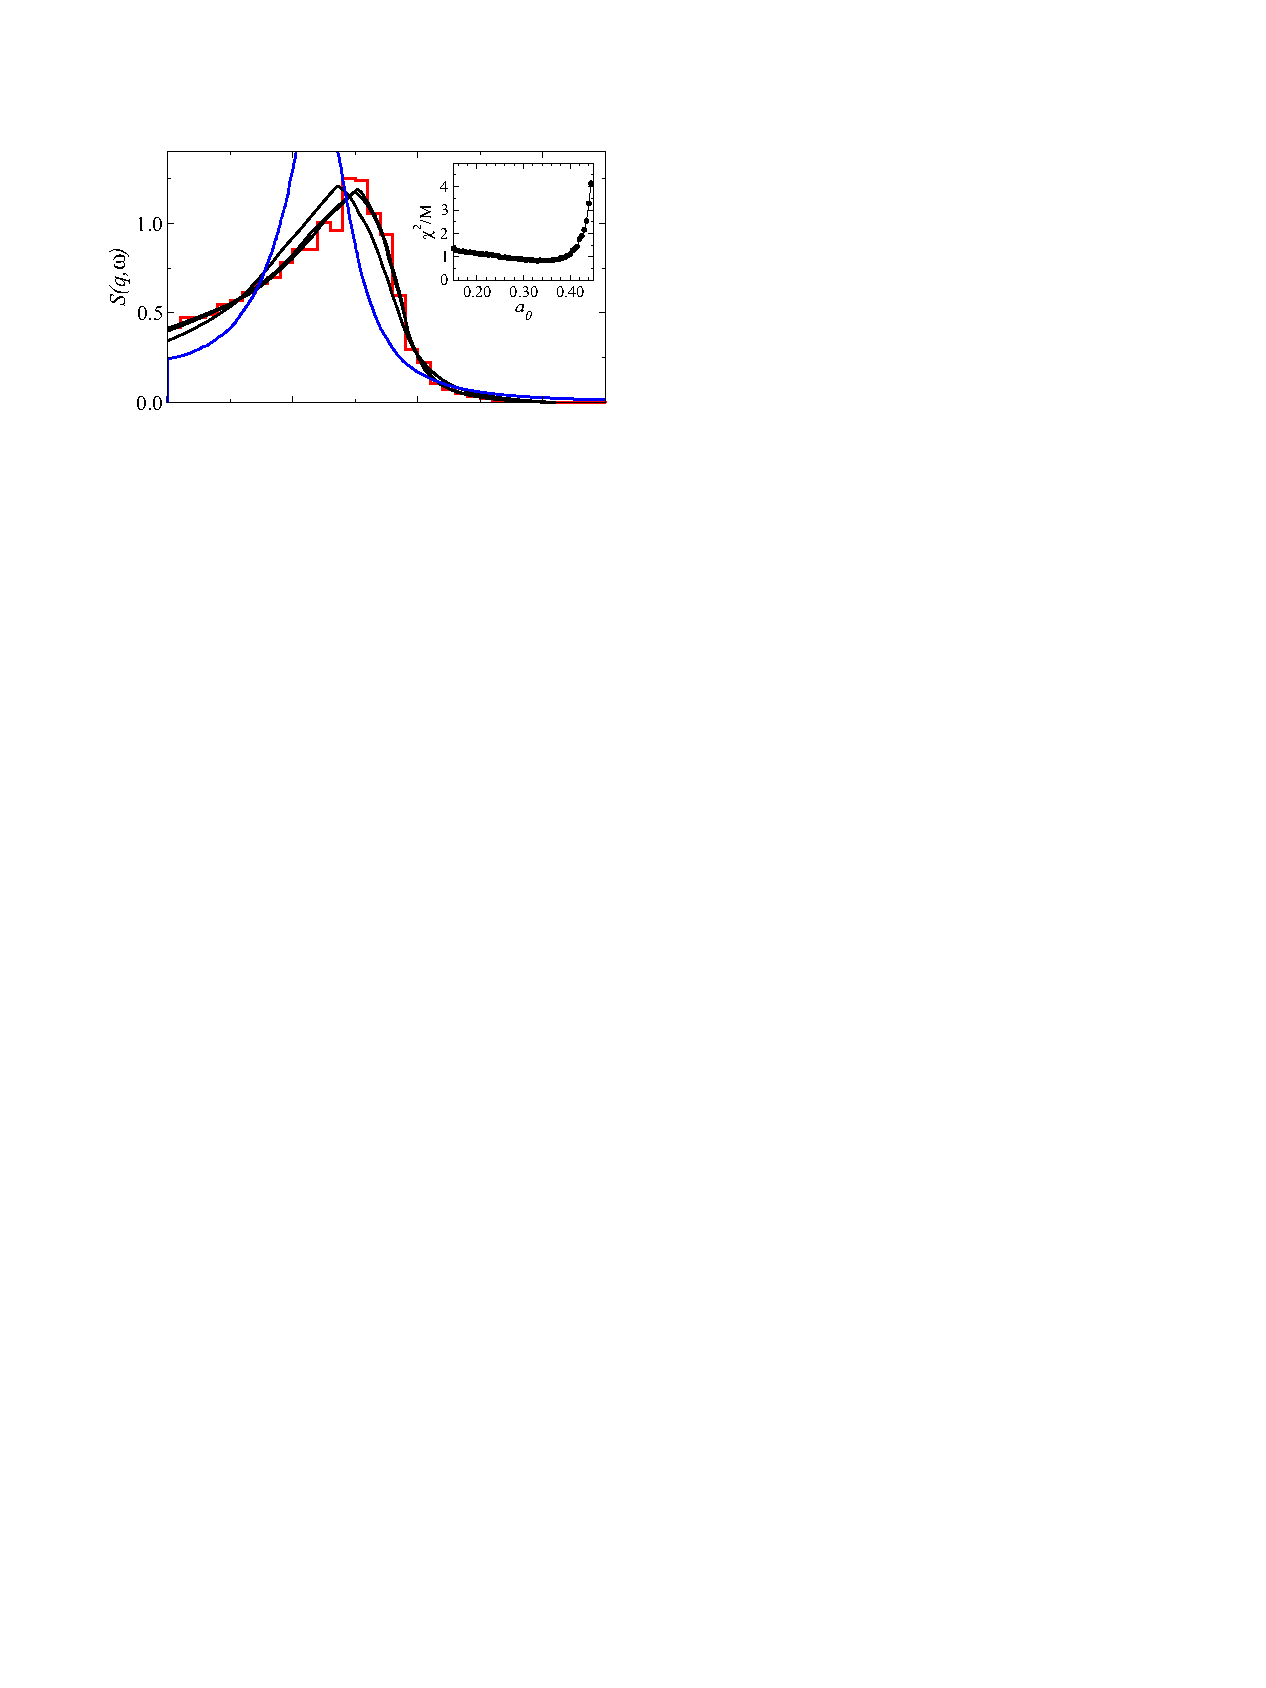
\includegraphics[height=3cm]{sac}}
  \end{center}
\end{frame}

\begin{frame}
  \frametitle{Fitting experiments}
  \[H = J_1\sum_{\langle ij\rangle}S_i^zS_j^z +J_2\sum_{\langle\langle ij\rangle\rangle}S_i^zS_j^z - \sum_i\left(\Delta S_i^x + h^zg_\parallel\mu_BS_i^z\right). \]
  Best fit is obtained at $J_1 = 0.99 \text{meV}$, $J_2 = 0.05J_1$,  $\Delta= 0.54J_1$ and $g_\parallel = 13.212$.
  \begin{center}
    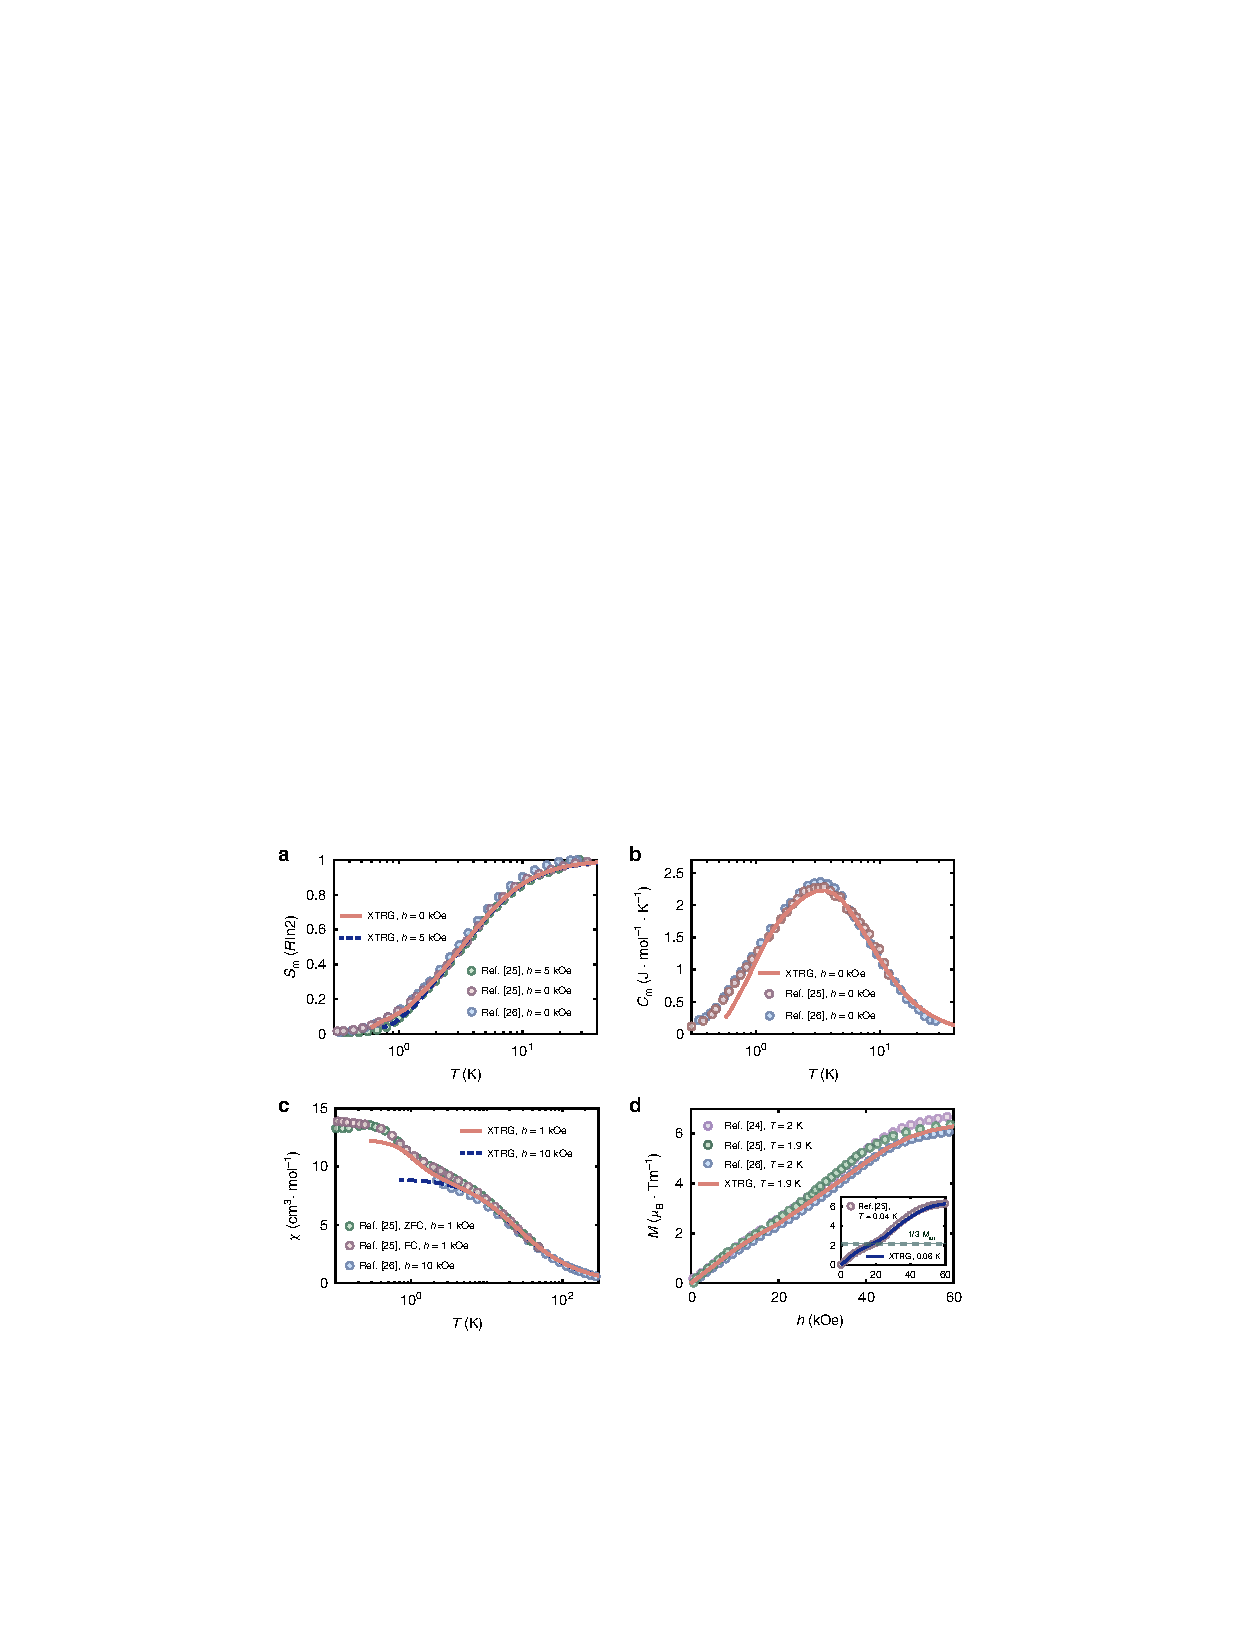
\includegraphics[scale=.75]{thermal-fit}
  \end{center}
\end{frame}

\begin{frame}
  \frametitle{Comparing with neutron scattering}
  \begin{itemize}
    \item[a] The parameters determined from thermodynamic measurements are used to compute spin spectrum.
    \item Agrees well with INS experiments in Yao Shen et al, Nat. Comm. (2019).
    \item[b] Spectrum computed from parameters determined by a simple spin-wave calculation.
    \item Does not agree with INS data: strong renormalization effect due to interactions.
  \end{itemize}
  \begin{center}
    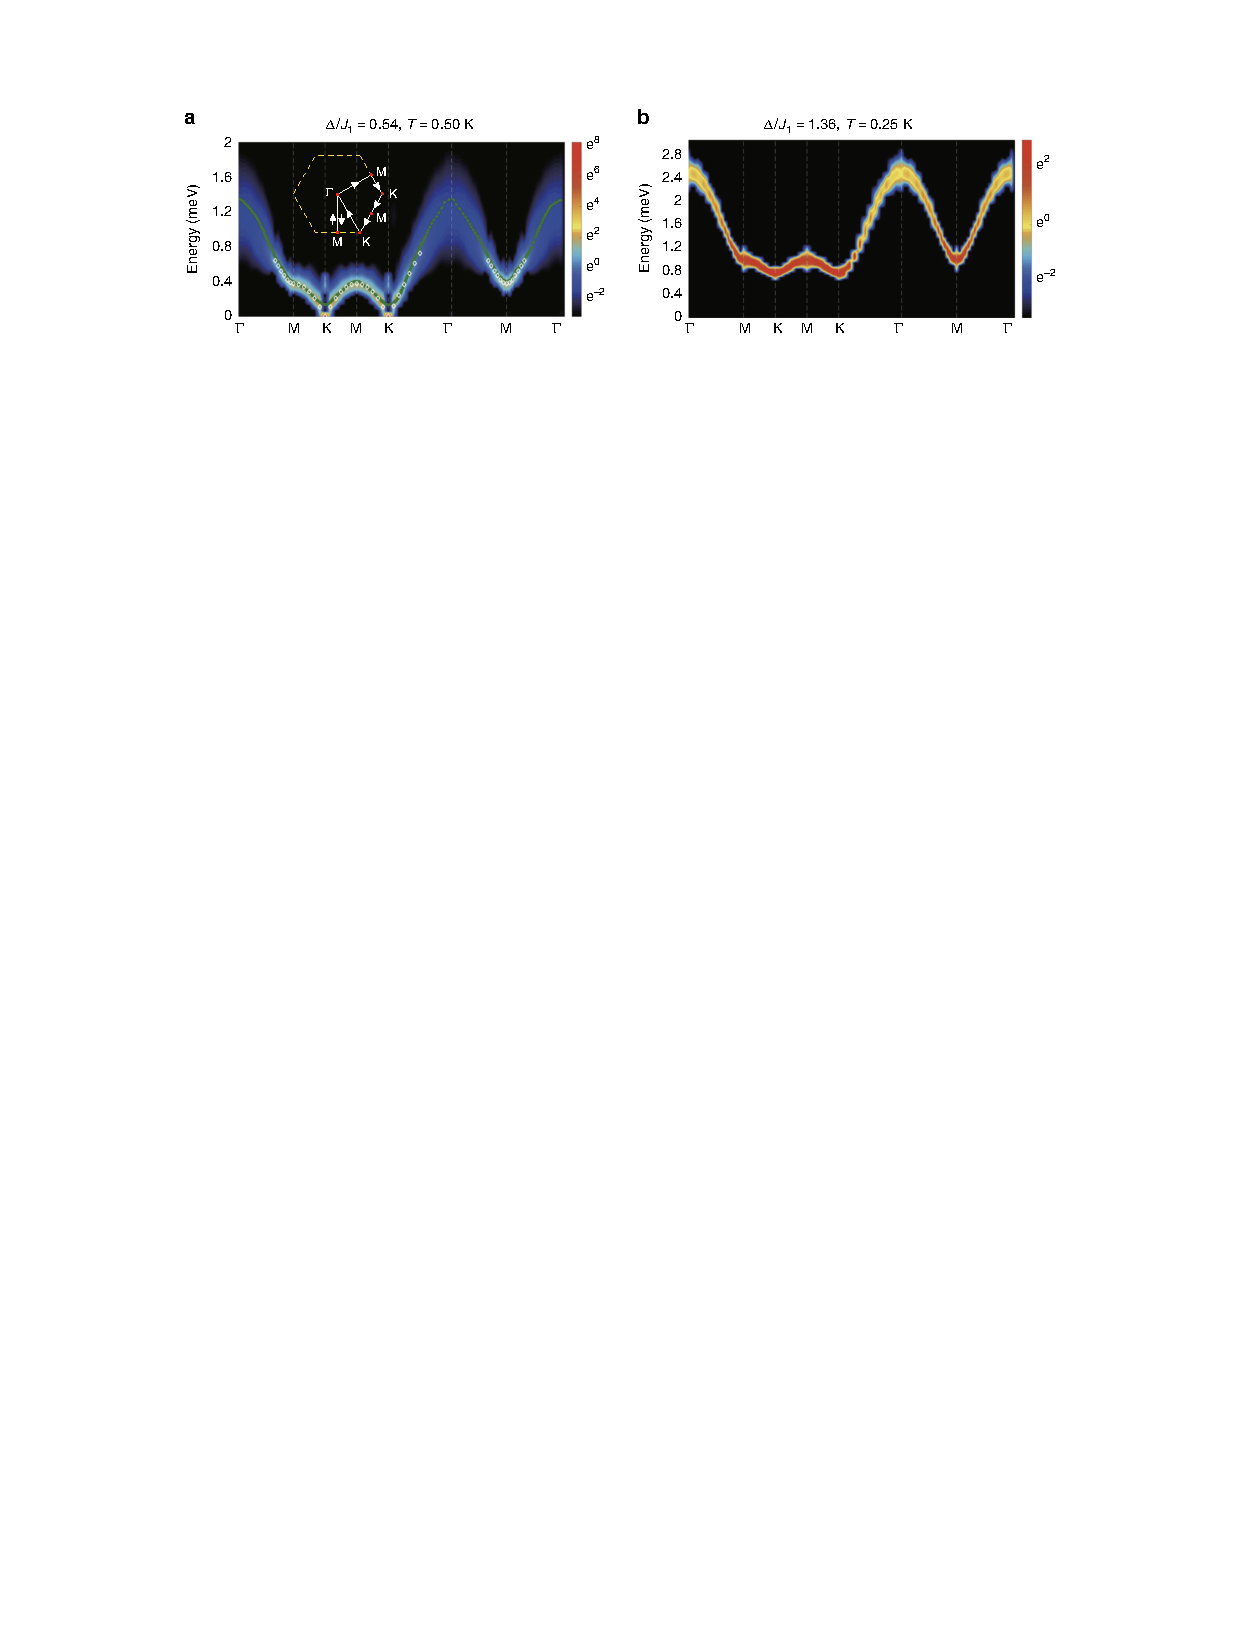
\includegraphics{spinwave-fit}
  \end{center}
\end{frame}

\section{Model: Emergent U(1) symmetry and BKT transitions}

\begin{frame}
  \frametitle{Why an Ising model hosts BKT transitions?}
  \begin{itemize}
    \item BKT transition happens at 2D + U(1) symmetry.
    \item Transverse-field Ising model (TFIM) only has discrete symmetries:
    \begin{itemize}
      \item $\mathbb Z_2$ spin-flip symmetry.
      \item p6mm wallpaper-group symmetry: containing 6-fold rotation.
    \end{itemize}
      %\item W/o $h$: classical ground state: massive ground-state degeneracy.
      %\item Degeneracy is lifted with quantum fluctuations introduced by $h$.
      \item Ground state: AFM, w/ 6-fold symmetry breaking. (Order-by-disorder)
  \end{itemize}
  \[H = J_1\sum_{\langle ij\rangle}S_i^zS_j^z +J_2\sum_{\langle\langle ij\rangle\rangle}S_i^zS_j^z - \sum_i\left(hS_i^x + h^zS_i^z\right). \]

  \begin{center}
    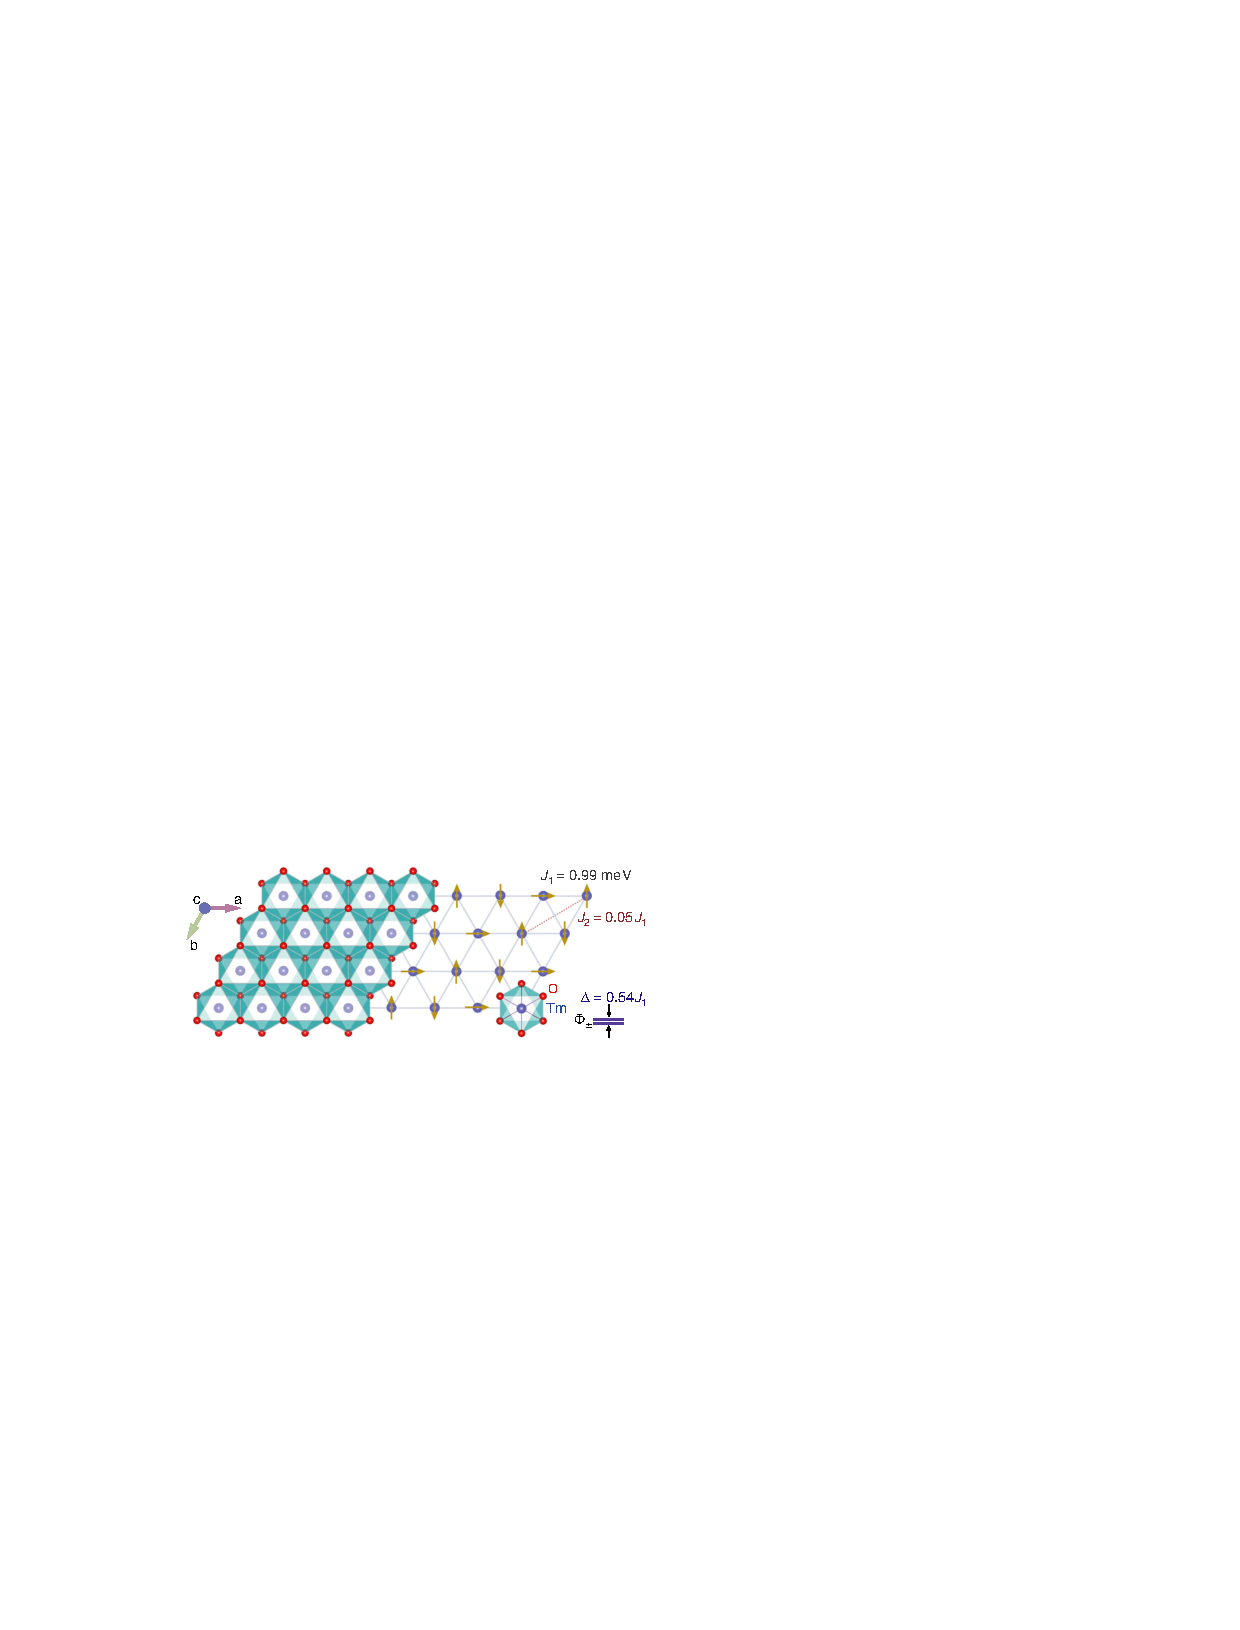
\includegraphics{lattice-afm}
  \end{center}
  {\footnotesize R Moessner and S L. Sondhi, Phys Rev B \textbf{63}, 224401 (2001).}
\end{frame}

%\begin{frame}
%  \frametitle{Emergent U(1) symmetry: a quantum example}
%  \begin{itemize}
%    \item \emph{Imagine} increasing $h$: quantum phase transition from AFM to PM.
%    \item Order parameter for the AFM phase:
%    \[m=|m|e^{i\theta} = m_1 + m_2e^{i2\pi/3} + m_3e^{i4\pi/3}.\]
%    \item $C_3$ action: $\theta\rightarrow\theta+\frac{2\pi}3$;
%    $\mathbb Z_2$ action: $\theta\rightarrow\theta+\pi$.
%    \item Ginzburg-Landau theory:
%    \[\mathcal L = |\partial_\tau m|^2+|\nabla m|^2 + r|m|^2 + u_4|m|^4 + u_6|m|^6+\alert{v_6|m|^6\cos(6\theta)}+\cdots.\]
%    \item $v_6$ is irrelevant: emergent U(1) symmetry.
%  \end{itemize}
%  \begin{center}
%    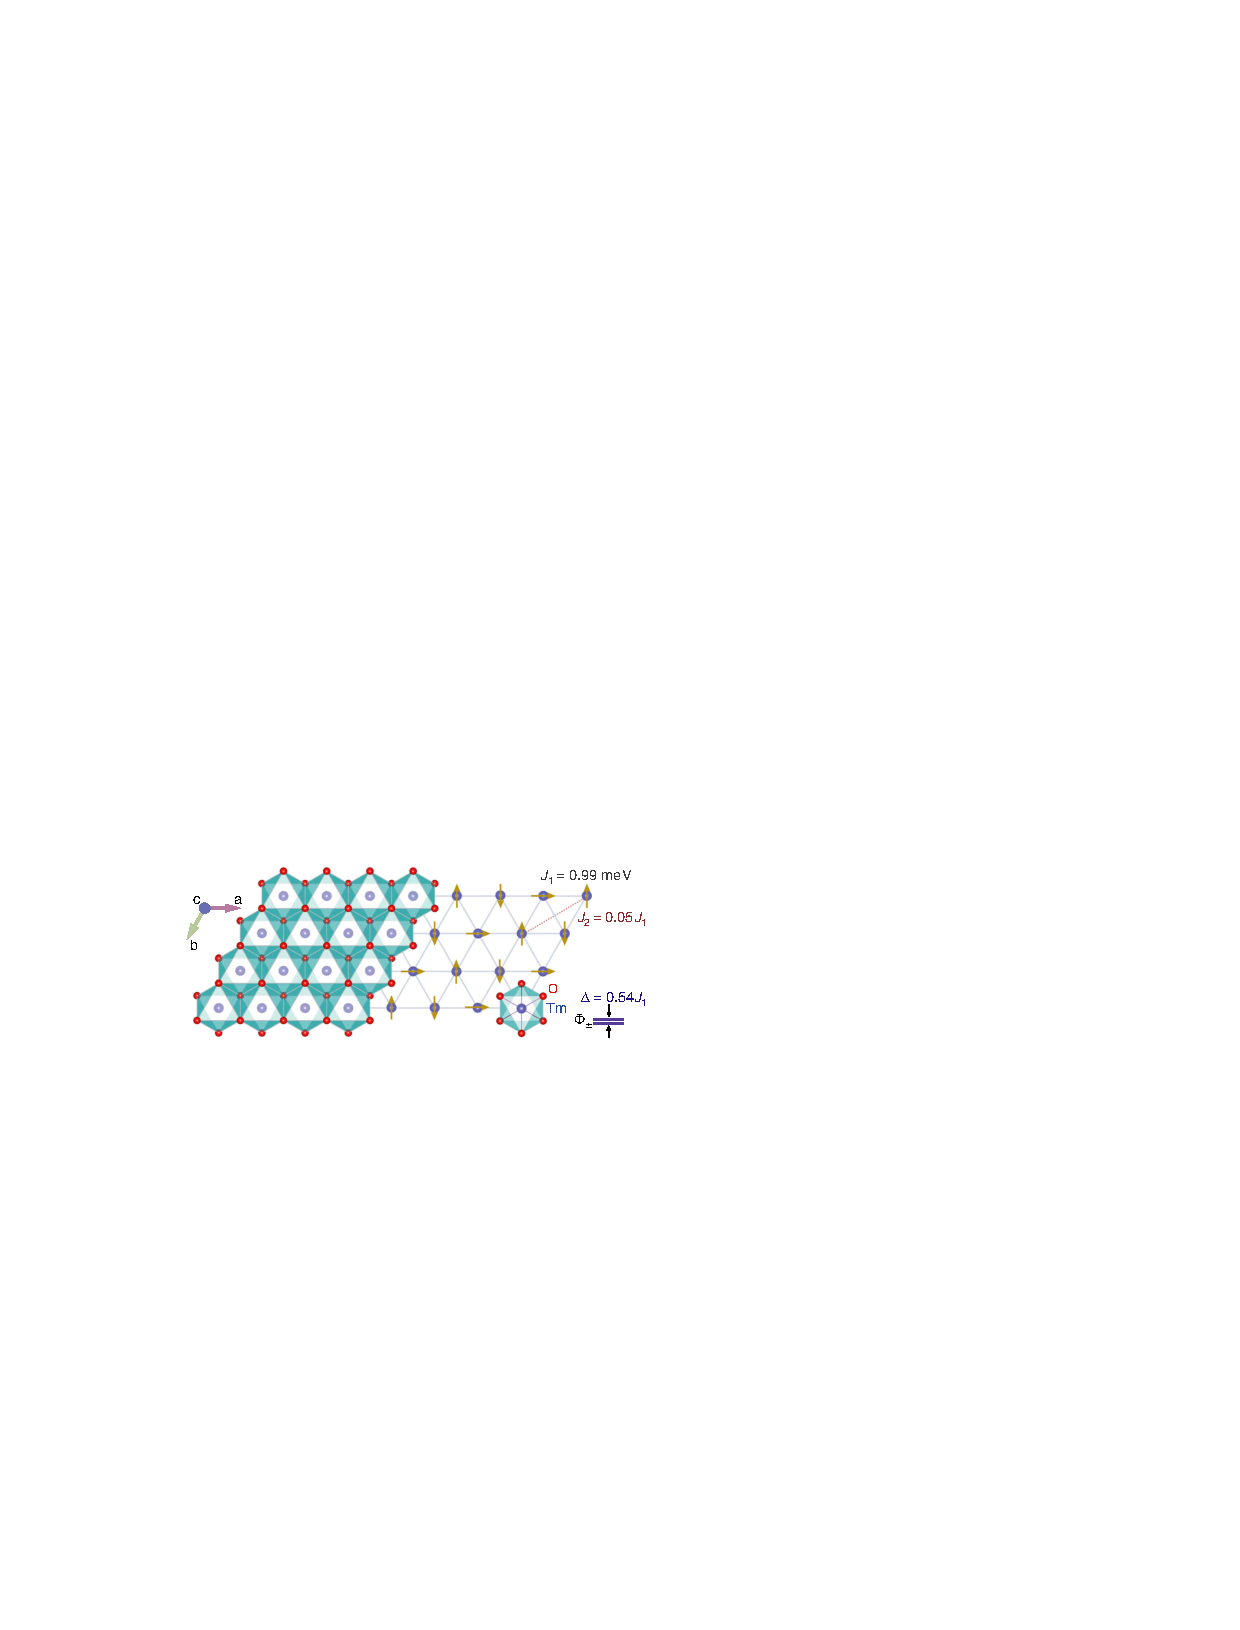
\includegraphics[height=2.5cm]{lattice-afm}~~~~
%    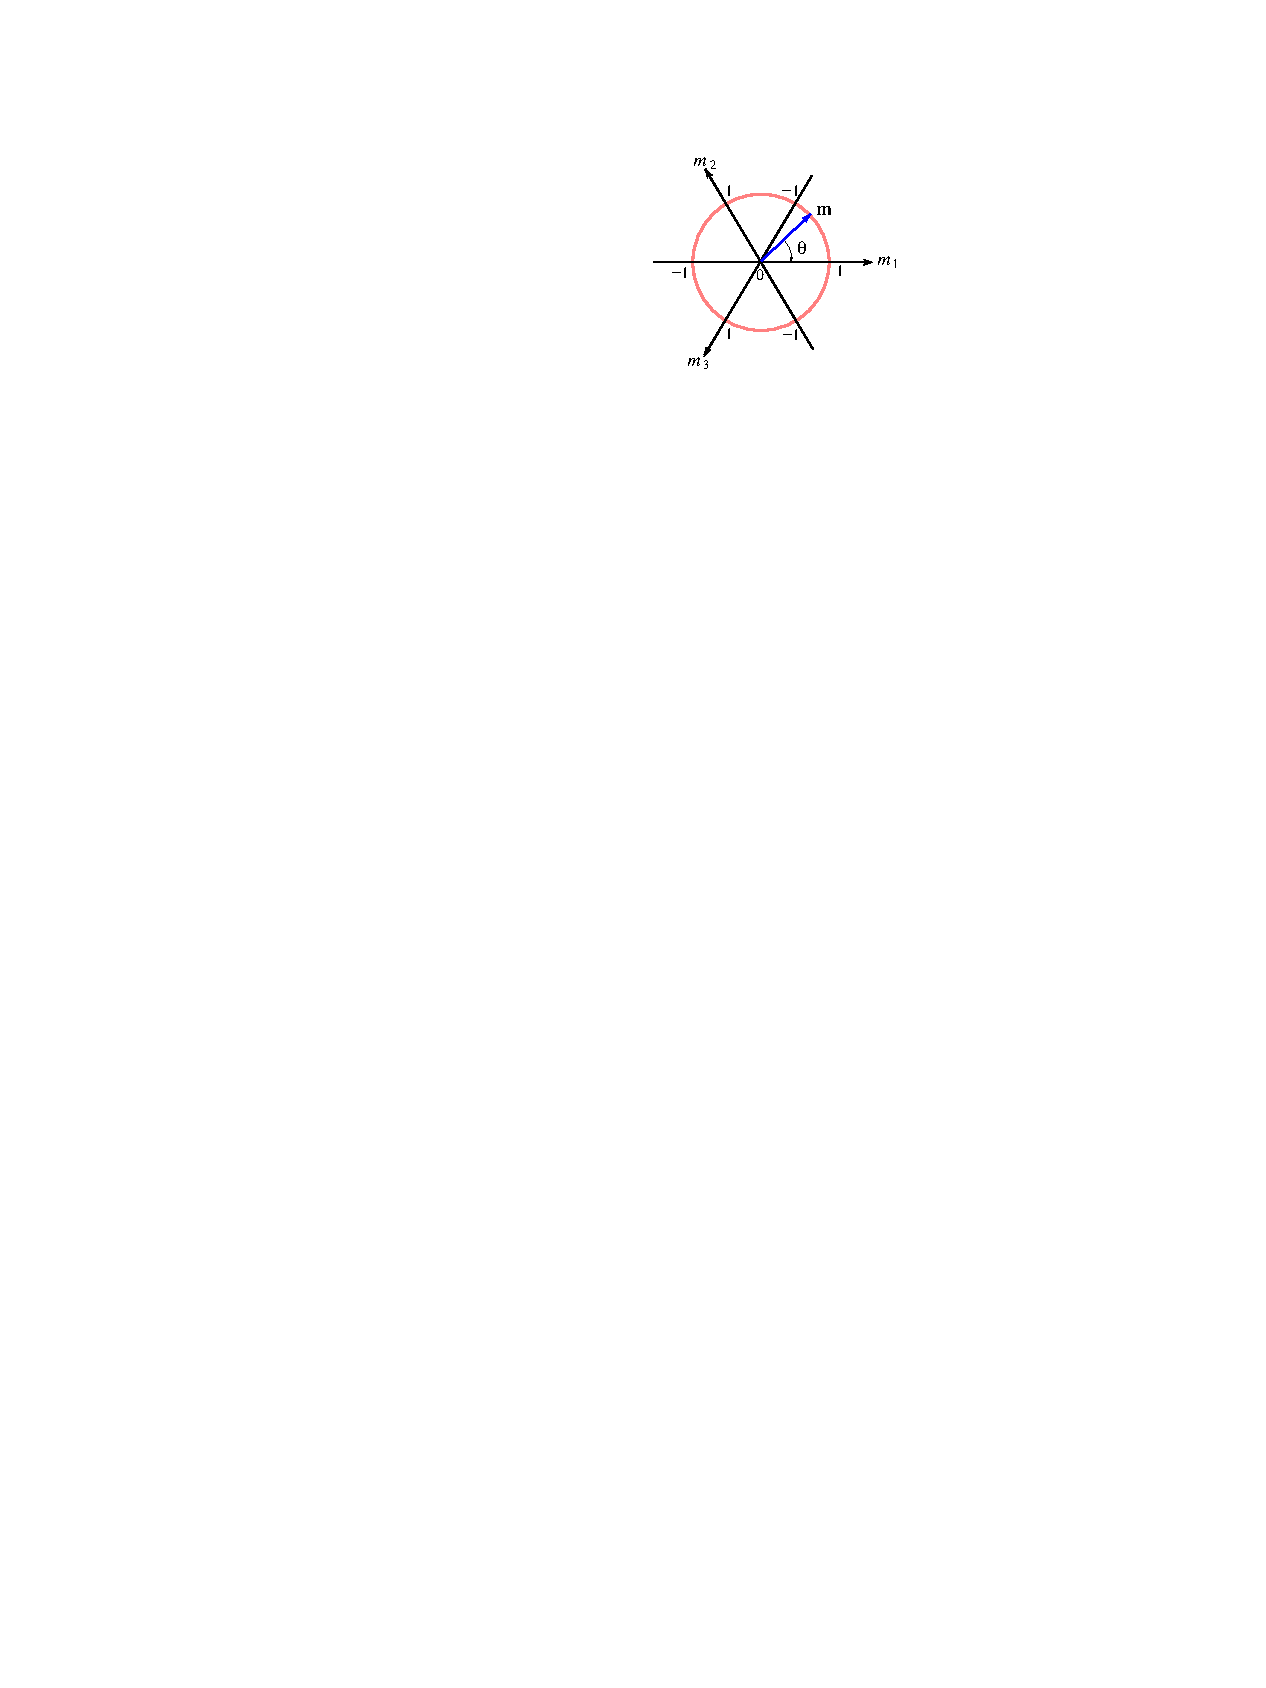
\includegraphics[height=2.5cm]{order-param}
%  \end{center}
%  {\footnotesize Isakov and Moessner, Phys Rev B \textbf{68}, 104409 (2003).}
%\end{frame}

\begin{frame}
  \frametitle{Emergent U(1) symmetry at finite temperatures}
  \begin{itemize}
    \item[?] Can we have emergent U(1) symmetry? U(1) symmetry + 2D = BKT.
    \item \alert{Assume} there is a BKT phase.
    \item Effective field theory: sine-Gorden model w/ 6-fold anisotropy.
    \[\mathcal L = \frac1{4\pi g}(\nabla\theta)^2 + v\cos(6\theta).\]
    \begin{itemize}
      \item $v$ is irrelevant when $g>\frac19$.
      \item Vortex is irrelevant when $g < \frac14$.
    \end{itemize}
    \item Indeed, a BKT phase at $\frac19<g<\frac14$, and two BKT transitions.
  \end{itemize}
  \begin{center}
    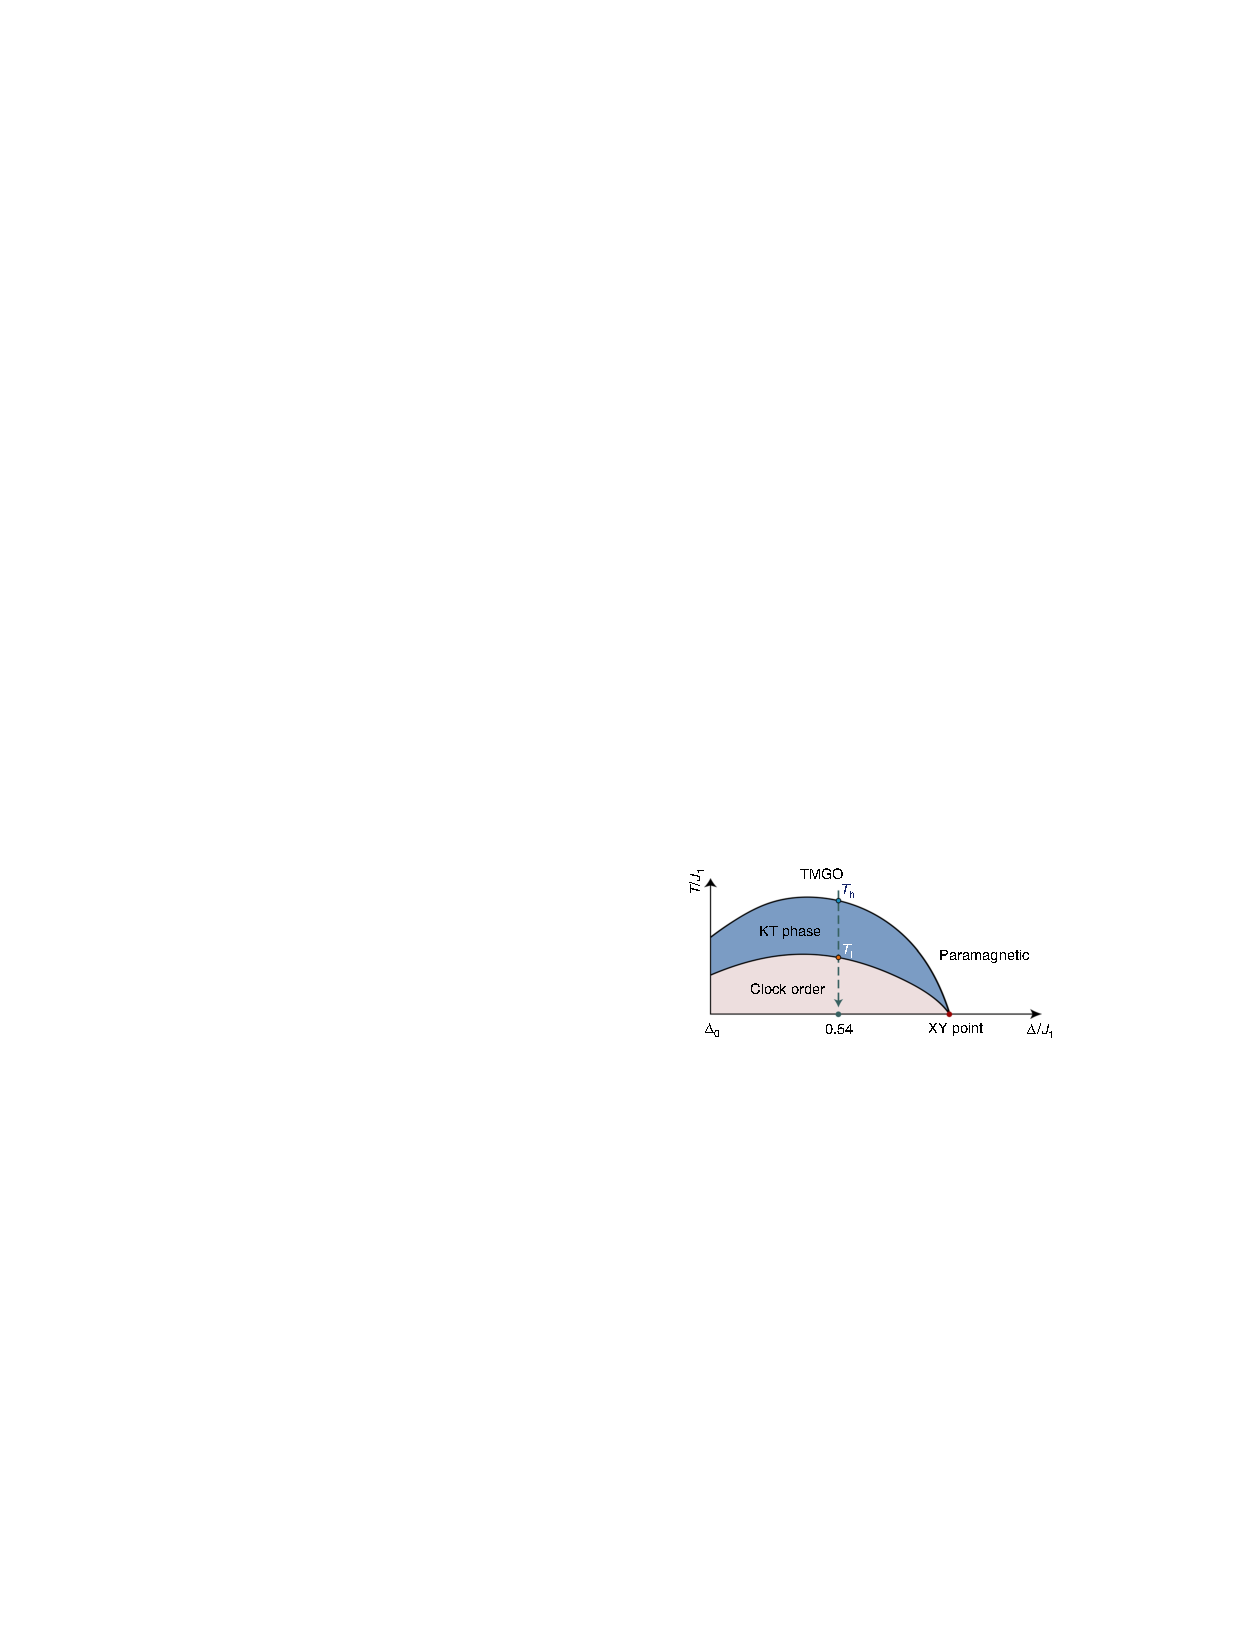
\includegraphics{phase-diagram}
  \end{center}
\end{frame}

\section{Experiment: Detecting the BKT phase using NMR relaxation time}

\begin{frame}
  \frametitle{Why we think NMR would work}
  \begin{enumerate}
    \item Prediction: a BKT phase and two BKT transitions.
    \item How to detect in experiments?
    \begin{itemize}
      \item BKT transitions have extremely weak singularities: infinite-order transitions.
      \item It is difficult to distinguish quasi-long-range and true long-range correlations.
    \end{itemize}
    \item NMR spin-lattice relaxation time $T_1$ measures gapless spin excitations
    \[\frac1{TT_1}\propto \sum_q|A(\bm q)|^2S(\bm q, \omega\rightarrow0^+)\]
    \item Sum over all momenta: allows us to see the physics at $K$.
    \item Applying a field in the $x$ direction does not perturb the model:
    $h$ is not $h_x$, and $h_x$ does not couple to the dipole-multipole moment.
  \end{enumerate}
  \begin{center}
    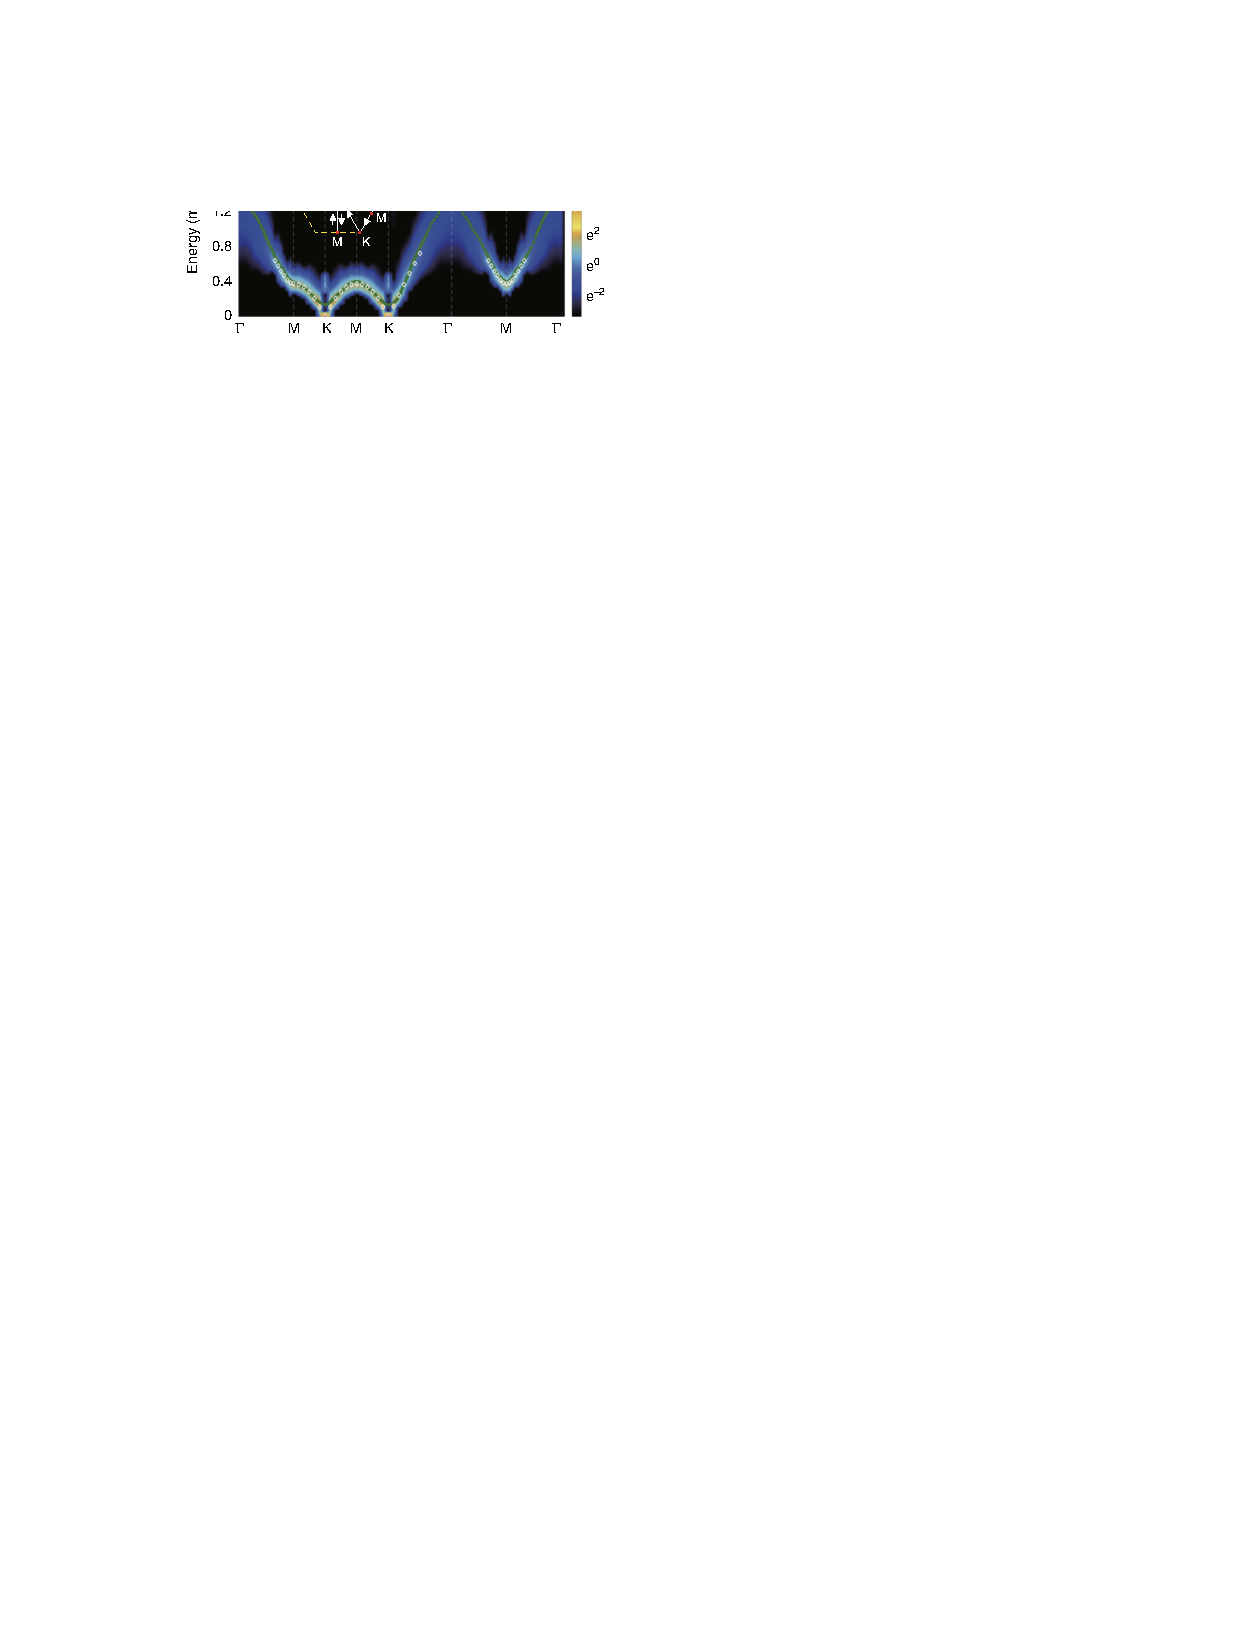
\includegraphics[width=.6\textwidth]{spinwave-fit1}
  \end{center}
\end{frame}

\begin{frame}
  \frametitle{Experiment and numerical simulations}
  \begin{columns}
    \column{.4\textwidth}
    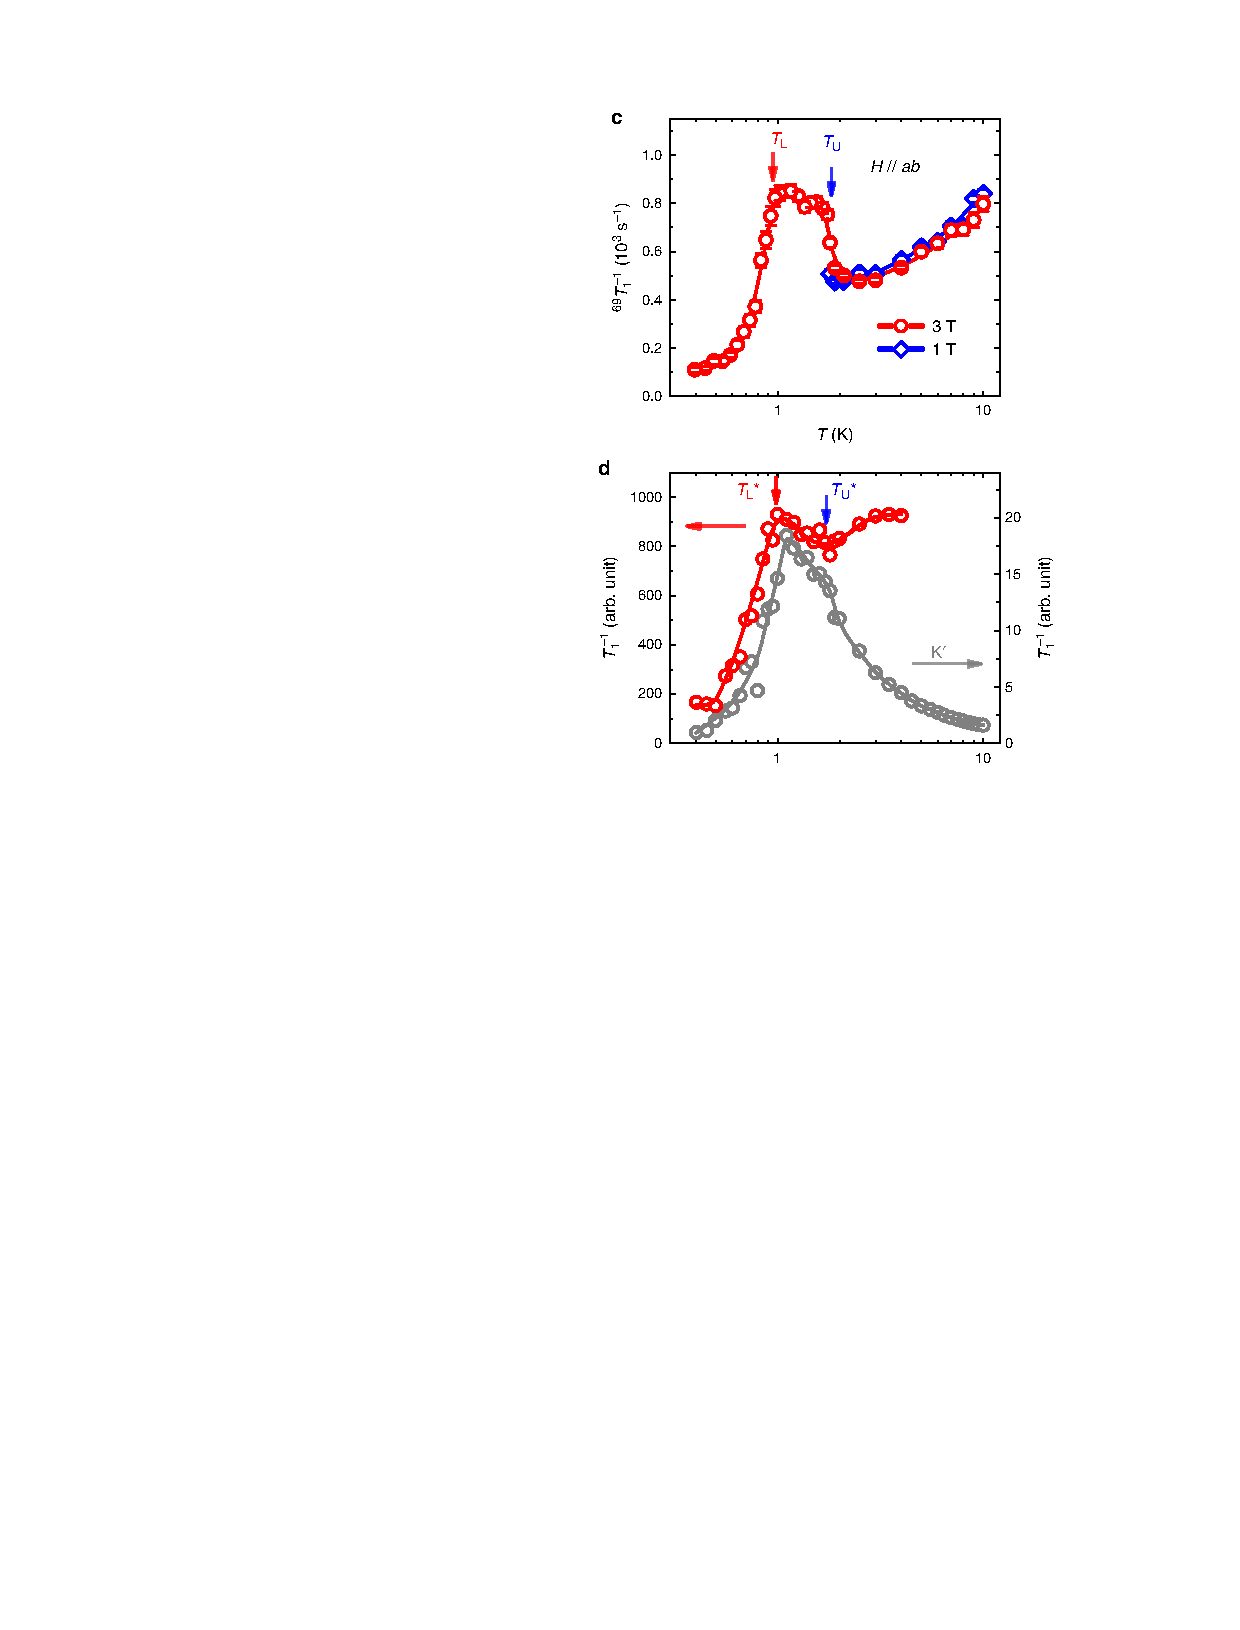
\includegraphics[height=8cm]{nmr}
    \column{.6\textwidth}
    \begin{itemize}
      \item No field dependence: $h_x$ does not couple to the effective spin.
      \item Plateau between $T_L\sim 0.9K$ and $T_U\sim1.9K$.
      \item BKT phase and transitions?
      \item QMC + SAC qualitatively reproduces the feature, despite of the unknown form factor.
    \end{itemize}
  \end{columns}
\end{frame}

\begin{frame}
  \frametitle{Conclusions}
  \begin{itemize}
    \item Effective model for TmMgGaO${}_4$:
    \[H = J_1\sum_{\langle ij\rangle}S_i^zS_j^z +J_2\sum_{\langle\langle ij\rangle\rangle}S_i^zS_j^z - \sum_i\left(h S_i^x + h^zg_\parallel\mu_BS_i^z\right). \]
    $J_1 = 0.99 \text{meV}$, $J_2 = 0.05J_1$,  $h= 0.54J_1$ and $g_\parallel = 13.212$.
    \item An emergent U(1) symmetry, a BKT phase and two BKT transitions.
    \item Evidence for BKT physics provided by NMR $T_1$ measurement.
  \end{itemize}
\end{frame}

\begin{frame}
  \frametitle{Remaining questions and future directions}
  \begin{itemize}
    \item Is $T_L$ and $T_U$ really the BKT transition temperatures?\\
    Fluctuations with diverging correlation lengths above the BKT transition.
    \item Comparing transition temperatures obtained in experiments and numerics: can our model describe physics at $T\rightarrow0$?
    \item Effect of disorders?
    \item How to directly measure BKT physics? Other experimental probes?
    \item Physics at $h_z>0$?
  \end{itemize}
\end{frame}

\end{document}
% !TEX engine = xelatex
%%% Local Variables:
%%% coding: utf-8
%%% mode: latex
%%% TeX-engine: xetex
%%% End:
